\documentclass{thesisclass}

%% -------------------------------
%% |    IM Thesis Template       |
%% -------------------------------
%% Additions by: David Dauer, IM, 2011
%% dauer@iism.uni-karlsruhe.de

%% Notes:
%% Language switch after \begin{document}

% Based on thesisclass.cls of Timo Rohrberg, 2009
% ----------------------------------------------------------------
% Thesis - Main document
% ----------------------------------------------------------------

%% ---------------------------------
%% |      Additional packages      |
%% ---------------------------------
%% 

\usepackage{graphicx}
%http://en.wikibooks.org/wiki/LaTeX/Importing_Graphics#Graphics_storage
\DeclareGraphicsExtensions{.pdf,.png,.jpg}
\graphicspath{{./figures/}} %Use curly braces for each path to add and don't
% forget trailing slash '/'
% \usepackage{epstopdf} %Nice to automatically convert eps figures to pdf
% format  (from inkscape, etc)


%% ---------------------------------
%% | Information about the thesis  |
%% ---------------------------------

\newcommand{\mytype}{\iflanguage{english}{Master Thesis}{Master-Arbeit}} % (Seminar|Bachelor|Master) Thesis
\newcommand{\myname}{Thomas Knapp}
\newcommand{\mytitle}{\iflanguage{english}{Title}{Entwicklung eines mobilen Software-Assistenten zur Unterst�tzung der vernetzten Pflege}}
\newcommand{\myinstitute}{\iflanguage{english}
{Institute of Information Systems and Management (IISM) \\
Information \& Market Engineering}
{Institut f�r Informationswirtschaft und -management (IISM) \\
Information \& Market Engineering}}

\newcommand{\reviewerone}{Prof. Dr. rer. pol. Christof Weinhardt}
\newcommand{\reviewertwo}{Dr. Henner Gimpel}
\newcommand{\advisor}{Bruno Rosales Saurer}
\newcommand{\advisortwo}{Mathias Schmon}
\newcommand{\advisorthree}{Imanol Bernabeu}

\newcommand{\timestart}{01. Oktober 2012}
\newcommand{\timeend}{31. M�rz 2012}
\newcommand{\submissiontime}{31. 03. 2012}

%% -------------------------------
%% |  Information for PDF file   |
%% -------------------------------
%% IM: Auto-Fill this information
\hypersetup{
 pdfauthor={\myname},
 pdftitle={\mytitle},
 pdfsubject={\mytype},
 pdfkeywords={\mytype}
}

%% ---------------------------------
%% | ToDo Marker - only for draft! |
%% ---------------------------------
% Remove this section for final version!
\setlength{\marginparwidth}{20mm}

\newcommand{\margtodo}
{\marginpar{\textbf{\textcolor{red}{ToDo}}}{}}

\newcommand{\todo}[1]
{{\textbf{\textcolor{red}{(\margtodo{}#1)}}}{}}


%% --------------------------------
%% | Old Marker - only for draft! |
%% --------------------------------
% Remove this section for final version!
\newenvironment{deprecated}
{\begin{color}{gray}}
{\end{color}}


%% --------------------------------
%% | Settings for word separation |
%% --------------------------------
% Help for separation:
% In german package the following hints are additionally available:
% "- = Additional separation
% "| = Suppress ligation and possible separation (e.g. Schaf"|fell)
% "~ = Hyphenation without separation (e.g. bergauf und "~ab)
% "= = Hyphenation with separation before and after
% "" = Separation without a hyphenation (e.g. und/""oder)

% Describe separation hints here:
\hyphenation{
% Pro-to-koll-in-stan-zen
% Ma-na-ge-ment  Netz-werk-ele-men-ten
% Netz-werk Netz-werk-re-ser-vie-rung
% Netz-werk-adap-ter Fein-ju-stier-ung
% Da-ten-strom-spe-zi-fi-ka-tion Pa-ket-rumpf
% Kon-troll-in-stanz
}


%% ------------------------
%% |    Including files   |
%% ------------------------
% Only files listed here will be included!
% Userful command for partially translating the document (for bug-fixing e.g.)
\includeonly{%
titlepage,
text/einleitung,
text/zieleArbeit,
text/anforderungsanalyse,
text/entwurfsentscheidungen,
text/plugins,
text/evaluation,
text/ausblick,
text/conclusion,
text/declaration,
text/appendix
}

%%%%%%%%%%%%%%%%%%%%%%%%%%%%%%%%%
%% Here, main documents begins %%
%%%%%%%%%%%%%%%%%%%%%%%%%%%%%%%%%
\begin{document}

% Comment the following line out for German text
% \selectlanguage{english}

\frontmatter
\pagenumbering{roman}
%% titlepage.tex
%%

% coordinates for the bg shape on the titlepage
\newcommand{\diameter}{20}
\newcommand{\xone}{-15}
\newcommand{\xtwo}{160}
\newcommand{\yone}{15}
\newcommand{\ytwo}{-253}

\begin{titlepage}
% bg shape
\begin{tikzpicture}[overlay]
\draw[color=gray]  
 		 (\xone mm, \yone mm)
  -- (\xtwo mm, \yone mm)
 arc (90:0:\diameter pt) 
  -- (\xtwo mm + \diameter pt , \ytwo mm) 
	-- (\xone mm + \diameter pt , \ytwo mm)
 arc (270:180:\diameter pt)
	-- (\xone mm, \yone mm);
\end{tikzpicture}
	\begin{textblock}{10}[0,0](4,2.5)
		\iflanguage{english}
			{
\includegraphics[width=.3\textwidth]{logos/KITLogo_EN_RGB.pdf}}
			{
\includegraphics[width=.3\textwidth]{logos/KITLogo_DE_RGB.pdf}}		
	\end{textblock}
	\begin{textblock}{10}[0,0](10,2.5)
		
\includegraphics[width=.6\textwidth]{logos/IISMLogo_RGB.pdf}
	\end{textblock}
	\changefont{ppl}{m}{n}	% helvetica	(phv), % IM Style: palatino (ppl) 
	\vspace*{3.5cm}
	\begin{center}
		\Huge{\mytitle}
		\vspace*{2cm}\\
		\Large{
			\iflanguage{english}{\mytype\\of}			
								{\mytype\\von}
		}\\
		\vspace*{1cm}
		\huge{\myname}\\
		\vspace*{1cm}
		\Large{
			\iflanguage{english}{At the Department of Economics and Business Engineering}			
							    {An der Fakult\"at f\"ur Wirtschaftswissenschaften}
			\\
			\myinstitute
		}
	\end{center}
\large{
\begin{center}
\begin{tabular}[ht]{l c l}
  % Gutachter sind die Professoren, die die Arbeit bewerten. 
  %\iflanguage{english}{Reviewer}{Erstgutachter}: & \hfill  & \reviewerone\\
  \iflanguage{english}{Reviewer}{Gutachter}: & \hfill  & \reviewerone\\
  %\iflanguage{english}{Second reviewer}{Zweitgutachter}: & \hfill  & \reviewertwo\\
  \iflanguage{english}{Advisor}{Betreuender Assistent}: & \hfill  & \reviewertwo\\
  Betreuende Mitarbeiter FZI:
  & \hfill  & \advisor\\
  & \hfill  & \advisortwo\\
  & \hfill  & \advisorthree\\
  % IM: No second advisor
  % Der zweite betreuende Mitarbeiter kann weggelassen werden. 
\end{tabular}
\end{center}
}


\vspace{1.5cm}
\begin{center}
\large{\timeend}
% \iflanguage{english}{Duration:}{Bearbeitungszeit:} \timestart \hspace*{0.25cm}
% -- \hspace*{0.25cm} 
% \timeend}
\end{center}


\begin{textblock}{10}[0,0](4,16.8)
\tiny{ 
	\iflanguage{english}
		{KIT -- University of the State of Baden-Wuerttemberg and National Laboratory of the Helmholtz Association}
		{KIT -- Universit\"at des Landes Baden-W\"urttemberg und nationales Forschungszentrum der Helmholtz-Gesellschaft}
}
\end{textblock}

\begin{textblock}{10}[0,0](14,16.75)
\large{
	\textbf{www.kit.edu} 
}
\end{textblock}

\end{titlepage}

% IM Style: No additional blank page
% \blankpage


%% -------------------
%% |   Directories   |
%% -------------------
\tableofcontents
% IM Style: No additional blank page
% \blankpage


%% -----------------
%% |   Main part   |
%% -----------------
\mainmatter
\pagenumbering{arabic}
%% introduction.tex
%%

%% ==============================
\chapter{Einleitung}
\label{ch:einleitung}
%% ==============================
\begin{itemize}
\item Kontext mit �rztemangel 
\item Als L�sungsansatz Delegation von Leistungen an qualitfiziertes Pflegepersonal ( wie werden MFPs ausgebildet???)
\item Effizienzsteigerung
\item Einbringen von Statistiken �ber Bev�lkerungsentwicklung, Demographiewandel
\end{itemize}

\cite{kopetsch2010}\\
dfgsdgsgsetgrtgstr

\dots


\chapter{Ziele der Arbeit}
\label{ch:zielederarbeit}
blub
\chapter{Analyse der Anforderungen und daraus abgeleitete Entwurfsentscheidungen}
\label{ch:anforderungsanalyse}

In diesem Kapitel werden die aus Literatur und vorangegangenen Projekten hervorgegangenen Anforderungen an eine mobile
Anwendung zur Dokumentation von �rztlich �bertragenen T�tigkeiten vorgestellt. In Abschnitt \ref{sec:analyse} werden
funktionelle Anforderungen beschrieben und technische Anforderungen daraus abgeleitet. Abschnitt
\ref{sec:entwurfsentscheidungen} stellt Entwurfsentscheidungen vor, die zur Realisierung der Anwendung getroffen wurden.

\section{Analyse der Anforderungen}
\label{sec:analyse}

Zu Beginn der Bearbeitungszeit der Master-Arbeit konnte kein Termin mit den eigentlichen Endnutzern der mobilen
Anwendung vereinbart werden, um eine direkte Anforderungserhebung durchzuf�hren. Aufgrund dessen musste zun�chst eine
Anforderungsanalyse auf Basis von Literatur, aktuellen und vorangegangenen Arbeiten erg�nzt um Gespr�che mit mit
sachkundigen Mitarbeitern von Kranken- und Pflegeeinrichtungen durchgef�hrt werden. Da die Grundlage f�r die
M�glichkeit, �rztliche T�tigkeiten an speziell geschulte Pflegekr�fte zu �bertragen, die Richtlinie des Gemeinsamen
Bundesausschusses basierend auf � 63 Abs. 3c SGB V ist, kann die Dokumentation der hier aufgelisteten �bertragbaren
Leistungen als Basisanforderung gesehen werden. Ein Problem ist aber, dass aus der Auflistung der T�tigkeiten nicht die
zu dokumentierenden Daten hervorgehen. Diese konnten in der Literatur jedoch nicht im Detail ermittelt werden, da
einige Leistungen medizinisches Fachwissen �ber deren Erbringung erfordern. Deswegen wurde zun�chst
angenommen, dass in der Regel eine Best�tigung, ob eine Leistung erbracht wurde, ausreicht, und sonnst nur die
Dokumentation von Blutdruck und Puls als wertbasierte Leistungen notwendig ist, sowie das Fotografieren von Wunden.
Weitere zu dokumentierende Werte konnten erst bei einem Treffen mit den Endnutzern ermittelt werden. Die Ergebnisse
werden in Kapitel \ref{sec:evalEndnutzer} vorgestellt.\\

Das Ausbildungsprogramm zu einer \ac{mfp} nimmt keine Einschr�nkung des Arbeitsgebietes vor. Eine Pflegekraft kann
somit sowohl station�r in einer Pflegeeinrichtung arbeiten, als auch im ambulanten Dienst t�tig sein, bei der die
jeweiligen Klienten besucht werden. Die mobile Anwendung ist folglich so zu gestalten, dass beide Einsatzbereiche
abgedeckt werden k�nnen. Es ist zu erwarten, dass die zu erbringenden Leistungen im station�ren und im ambulanten
Bereich die gleichen sein werden, jedoch k�nnen sich Unterschiede bei den technischen Anforderungen oder der
Terminologie ergeben. Wird im Folgenden keine explizite Unterscheidung zwischen ambulanten und station�ren Anforderungen
genannt, so gilt eine Anforderung f�r beide Bereiche.\\

Jede �rztlich �bertragene T�tigkeit kann direkt einer Person zugeordnet werden. Um eine Interaktion mit der Person zu
erm�glichen, m�ssen bestimmte Daten �ber diese verf�gbar sein. Hierzu geh�ren Stammdaten wie Name, Adresse, Anschrift
und Alter, medizinische Daten �ber aktuell verabreichte Medikamente, Vorerkrankungen oder Allergien sowie Angaben zu
Angeh�rigen, dem zust�ndigen Hausarzt und einer eventuellen Pflegebed�rftigkeit. Aus der Notwendigkeit der Verf�gbarkeit
pers�nlicher Daten ergibt sich die Anforderung, diese Daten ausreichend zu sch�tzen und nur dem jeweiligen
Pflegepersonal zur Verf�gung zu stellen. Folglich muss eine Authentifizierungsfunktion in Form einer Anmeldung mit
Benutzername und Passwort (Log-In) implementiert werden. Ein Log-In erm�glicht es au�erdem, der angemeldeten Pflegekraft
nur die Informationen anzuzeigen, die sie f�r die Ausf�hrung ihrer T�tigkeit ben�tigt (Autorisierungsfunktion). So kann
ausgeschlossen werden, dass Informationen �ber Klienten verf�gbar sind, die gerade nicht behandelt werden.\\
Es wird angenommen, dass Pflegekr�fte in Schichten arbeiten, da eine Versorgung von Klienten Tag und Nacht gew�hrleistet
sein muss. Weiter wird angenommen, dass jede Pflegekraft w�hrend einer Schicht f�r eine bestimmte Anzahl von Klienten
zust�ndig ist, f�r die eine Menge vordefinierter Leistungen erbracht werden muss. Zu Beginn jeder Schicht bekommt eine
Pflegekraft einen Plan ausgeh�ndigt, in dem die abzuarbeitenden Stationen und die entsprechenden Leistungen aufgelistet
sind. In diesem Plan muss jede Leistung dokumentiert werden (vgl. \cite[S. 18 ff.]{diplChristina}). Eine Leistung wird
entweder durch das Setzen eines Hakens dokumentiert (Best�tigung) oder durch die Eintragung von Messwerten,
beispielsweise im Falle der Erfassung von Blutdruck und Puls. Ziel der mobilen Anwendung ist es, dass sowohl die
�bermittlung des Tagesplanes pro Pflegekraft als auch die Dokumentation der Leistungen elektronisch erfolgt. In einer
�bersicht �ber alle Klienten/Stationen sollte direkt erkennbar sein, ob bereits alle Leistungen einer Station erbracht
wurden, ohne die Einzelleistungen kontrollieren zu m�ssen.\\
Konnte eine Leistung nicht oder nicht vollst�ndig erbracht werden, muss es die M�glichkeit geben, dies zu dokumentieren.
Neben einer Markierung der Leistung muss ein Feld f�r eine Begr�ndung (Freitext oder mit vordefinierten Bausteinen)  der
Nichterbringung der Leistung verf�gbar sein. In der �bersicht �ber die Stationen einer Schicht sollte neben den
Zust�nden "`Erledigt"' und "`Offen"' au�erdem der Zustand "`Unvollst�ndig abgeschlossen"' ersichtlich sein, um zu
zeigen, dass zwar alle Leistungen bearbeitet wurden, jedoch nicht alle erbracht werden konnten.\\
Bei der manuellen Dokumentation kann es immer wieder zu Fehlern kommen. Beispielsweise wenn Werte falsch eingetragen
oder Leistungen best�tigt werden, die eigentlich noch nicht vollst�ndig erf�llt sind. Da diese Fehler auch mit einer
elektronischen Dokumentation nicht ausgeschlossen werden k�nnen, m�ssen einmal dokumentierte Leistungen stornierbar und
korrigierbar sein, ohne dass im zentralen System eingegriffen werden muss. Um einer Verf�lschung von
Dokumentationsergebnissen durch nachtr�gliche Ver�nderungen beispielsweise von Messwerten entgegen zu wirken, sollte
protokolliert werden, wer zu welchem Zeitpunkt eine �nderung vornimmt. Diese Protokollfunktion muss zur vollst�ndigen
�berwachung auch im zentralen System verf�gbar sein und mit der mobilen Anwendung synchron gehalten werden.\\
Vor allem im ambulanten Bereich kann es immer wieder vorkommen, dass Klienten in Gegenden besucht werden m�ssen, in
denen kein mobiles Internet verf�gbar ist. Da der Datenaustausch zwischen mobiler Anwendung und zentralem
Verwaltungssystem �ber eine Internetverbindung geschieht, w�re somit die Arbeit mit dem mobilen System nicht m�glich.
Darauf zu setzen, dass beim Klienten vor Ort eine lokale Internetverbindung genutzt werden kann, ist auch keine
praktikable L�sung, da die Wahrscheinlichkeit f�r Probleme mit der Einrichtung und Verf�gbarkeit hoch ist. Vor Ort beim
Klienten anzukommen und festzustellen, dass der Plan der zu erbringenden Leistungen wegen Verbindungsproblemen nicht
verf�gbar ist, f�hrt zu nicht hinnehmbaren Einschr�nkungen, da so eventuell wichtige medizinische T�tigkeiten nicht
durchgef�hrt werden. Notwendig ist deshalb, den Plan f�r eine oder mehrere Schichten sowie alle relevanten Informationen
zu Personen (Klienten, Angeh�rigen, �rzten) vor dem Beginn einer Schicht lokal auf dem mobilen Endger�t zu speichern und
somit auch ohne Internet verf�gbar zu haben. Lediglich Aktualisierungen m�ssten so w�hrend einer Schicht nachgeladen
werden. Wird das initiale Laden von Informationen �ber ein lokales Netzwerk durchgef�hrt, spart dies au�erdem
Datenvolumen ein, welches bei Vertr�gen mit Internet �ber das Mobilfunknetz meist sehr begrenzt ist
\textcolor{red}{(Quelle notwendig?)}.\\

Wichtig bei der Dokumentation von Wunden ist neben einer textuellen Beschreibung eine bildliche Erfassung. Dies k�nnte
mit einer mitgef�hrten Digitalkamera erfolgen, jedoch besteht dann das Problem, dass die aufgenommenen Bilder nach
vollendeter Schicht manuell an das zentrale System �bertragen werden m�ssen und den richtigen Patienten zugeordnet. Dies
kostet verh�ltnism��ig viel Zeit und kann zu Fehlern bei der Zuordnung f�hren. W�nschenswert ist deswegen eine Funktion
in der mobilen Anwendung, die es erm�glicht, direkt �ber eine interne Kamera Wundfotos aufzunehmen und diese an das
zentrale System zu �bertragen.\\
Eine �hnliche Anforderung wurde bei der Erfassung der Vitalwerte wie Puls und Blutdruck identifiziert. Neben der
manuellen Messung und Eintragung der ermittelten Werte g�be es die M�glichkeit, ein automatisches Messger�t via
Bluetooth an das mobile Endger�t anzuschlie�en und damit die Messung und Eintragung vollst�ndig zu automatisieren. Dass
dies grunds�tzlich m�glich ist, wurde im Projekt \textit{Stroke Manager} des \ac{fzi} gezeigt \cite{bluetoothPuls}. Die
automatische Erfassung w�rde Fehler bei der manuellen Eintragung von Messwerten w�rden somit ausgeschlossen.
Da die M�glichkeit besteht, dass das automatische Messger�t ausf�llt, muss eine manuelle Eintragung jedoch trotzdem
m�glich sein.\\
Das Projekt VitaBit befasste sich, �hnlich wie diese Arbeit, mit der Dokumentation von Pflegeleistungen ambulanter
Dienste. Auch hier musste einer Pflegekraft ein Tages-/Tourenplan angezeigt werden. Da die Leistungen ambulanter Dienste
ausschlie�lich vor Ort beim Klienten erbracht werden, die h�ufig allein leben und nur noch eingeschr�nkt mobil sind, hat
die Pflegekraft in der Regel einen Schl�ssel zu den Wohnr�umen des Klienten. Die Schl�ssel aller Klienten werden meist
an einem Bund zusammengefasst und mit Nummern zur Zuordnung versehen. Damit die Pflegekraft nicht erst lang nach dem
passenden Schl�ssel suchen muss, war eine Anforderung, dass die Schl�sselnummer direkt in der �bersicht der Stationen
auftaucht. Da die in dieser Arbeit entwickelte Arbeit ebenfalls f�r den ambulanten Pflegedienst gedacht ist, wird diese
Anforderung auch hier �bernommen. Im Falle der station�ren Betreuung von Klienten soll anstatt einer Schl�sselnummer die
Zimmernummer in der Einrichtung angezeigt werden.\\
Die Zielgruppe, f�r die die mobile Anwendung entwickelt wird, sind Angeh�rige der Alten- und Pflegeberufe. Da es sich
bei dieser Gruppe in der Regel um wenig IT-affine Personen handelt, muss die Anwendung �bersichtlich strukturiert werden
und intuitiv bedienbar sein, damit die H�rden der Benutzung durch die Bedienbarkeit m�glichst gering sind. Ziel ist es,
dass das grunds�tzliche Wissen �ber die Bedienung von Tablet-PCs sowie das Fachwissen �ber die Dokumentation der
Leistungen ausreicht, um die mobile Anwendung zu verwenden. Der Aufwand f�r Schulungen soll so minimal gehalten werden.
Konzeptionell soll eine Orientierung an den graphischen Benutzerschnittstellen von iOS und Android stattfinden, den
Betriebssystemen f�r mobile Ger�te von Apple und Google.\\
Eine Funktionalit�t, die in erster Linie f�r ambulante Pflegedienste interessant ist, ist die M�glichkeit die Adresse
eines Klienten auf einer Karte anzeigen zu lassen. Alternativ k�nnte \ac{gps} k�nnte auch die aktuelle Position relativ
zur Adresse des Klienten angezeigt werden, um eine Routenplanung durchzuf�hren und somit Fahrzeiten besser absch�tzen zu
k�nnen. Hierzu ist allerdings eine aktive Internetverbindung notwendig. Eine vollst�ndige Navigation ist nicht
geplant.\\
Um eine Reduzierung der elektronischen Ger�te zu erreichen, die eine Pflegekraft mitf�hren muss, ist eine Funktion zum
F�hren von Telefongespr�chen hilfreich. Einerseits k�nnten normale Telefongespr�che beispielsweise mit der Zentrale,
Angeh�rigen oder �rzten gef�hrt werden, andererseits w�re es aber auch m�glich, einen Notruf-Knopf in die Anwendung zu
integrieren, um in Notsituationen direkt Hilfe anfordern zu k�nnen. Beschr�nkt wird die Funktionalit�t zwar durch die
Notwendigkeit der Verf�gbarkeit eines Mobilfunknetzes, jedoch kann diese Einschr�nkung ebenso beim Mitf�hren eines
separaten Mobiltelefons.\\

Von der bisher beschriebenen Menge an Funktionen ist lediglich die automatische Erfassung von Blutdruck und Puls mittels
eines per Bluetooth angeschlossenen Messger�tes durch manuelle Erfassung substituierbar. Alle anderen Anforderungen
m�ssen auf Basis der in der Literatur gewonnen Erkenntnisse umgesetzt werden, um einen sinnvollen Einsatz der mobilen
Anwendung �berhaupt erst zu erm�glichen.\\

Aus den beschriebenen funktionalen Anforderungen an die mobile Anwendung ergeben sich eine Reihe von technischen
Anforderungen an das Endger�t. Grundanforderung ist eine Internetverbindung sowohl �ber ein lokales \ac{wlan}, als
auch �ber ein Mobilfunknetz, um Tourendaten und Aktualisierungen empfangen und senden zu k�nnen. Zur Dokumentation von
Wunden per Foto muss eine Kamera mit einer ausreichend hohen Aufl�sung vorhanden sein, damit das medizinische Personal
bei der Beurteilung der Wunden nicht durch schlechte Bildqualit�t eingeschr�nkt wird. Zur Unterst�tzung der intuitiven
Bedienung sollte das mobile Ger�t einen ber�hrungsempfindlichen Bildschirm haben, was aber bei allen Ender�ten der Fall
sein sollte, da dies eines der Hauptmerkmale von Tablet-PCs ist. Zur Bestimmung der Position einer Pflegekraft, um die
Route zum n�chsten Klienten zu berechnen, muss eine \acs{gps}-Verbindung m�glich sein. Sollen Messger�te f�r Blutdruck
und Puls angeschlossen werden, muss eine Bluetooth-Verbindung verf�gbar sein.

Da Alten- und Krankenpflege dem sozialen Bereich zuzuordnen ist und ein Ziel die Einsparung von Kosten ist,
sollten die Endger�te m�glichst geringe Kosten verursachen. Obwohl grunds�tzlich Tablet-PCs sowohl mit dem
Android-Betriebssystem als auch mit iOS die technischen Anforderungen erf�llen, k�nnen Android Ger�te im Schnitt zu
einem deutlich niedrigeren Preis erworben werden \textcolor{red}{[QUELLE]}. Aus diesem Grund f�llt die Entscheidung bei
der Wahl der Plattform auf Android.



\section{Entwurfsentscheidungen des Gesamtsystems auf Basis der erhobenen Anforderungen}
\label{sec:entwurfsentscheidungen}

Zur Dokumentation von Pfleget�tigkeiten auf Tablet-PC-�hnlichen Endger�ten arbeitete Christina Hardt
\cite{diplChristina} in Ihrer Diplomarbeit mit der im Projekt VitaBIT (\cite{vitaBitAerzteblatt} und
\cite{vitaBithaeuslich}) entwickelten Software. Diese bietet bereits Datenstrukturen f�r Tourenpl�ne und die Definition
von zu erledigenden T�tigkeiten pro Station. Da die Anforderungen dieser Arbeit auch Touren- bzw. Schichtpl�ne
ben�tigen, um diese auf einem Tablet-PC abrufen und anzeigen zu k�nnen, wird VitaVBIT die Basis f�r das in Kapitel
\ref{ch:ziele} beschriebene zentrale System darstellen. Da es im Kontext dieser Arbeit aber nicht mehr
um die Dokumentation von Pfleget�tigkeiten geht, sondern um die effiziente �bertragung �rztlicher T�tigkeiten an
Pflegepersonal, m�ssen �nderungen an VitaBIT vorgenommen werden. Um den �nderungen und dem Kontext der vernetzten Pflege
auch namentlich gerecht zu werden, wurde das zentrale System in CareNet (Care = Pflege, Net = Netz) umbenannt.\\

\begin{figure}
	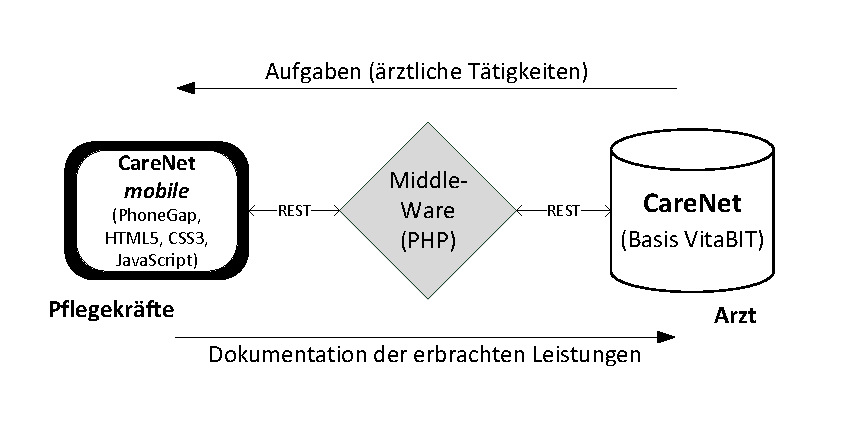
\includegraphics{figures/VerwendeteTechnologienGesamtsystem.pdf}
	\caption{Verwendete Technologien in der Gesamtarchitektur}
	\label{fig:technologien}
\end{figure}

Abbildung \ref{fig:technologien} zeigt die Komponenten des Gesamtsystems erweitert um die verwendeten
Technologien, auf denen diese basieren. Die Kommunikation zwischen den Komponenten erfolgt via Internet
mittels \acs{rest}. \acs{rest} steht f�r \textit{\acl{rest}} und stellt einen Architekturstil zur zustandslosen
Interaktion dar. Im Gegensatz zu aufwendigen Sitzungen (Sessions), die von Servern w�hrend der Interaktion mit einem
Benutzer verwaltet werden m�ssen, werden bei dem REST-Prinzip vorberechnete Ressourcen, beispielsweise eine Webseite,
�ber eine \acs{uri} (\acl{uri}) referenziert und geladen. Alle Informationen �ber den Kontext einer Anfrage sind in der
Anfrage selbst enthalten und es werden keine weiteren lokal beim Nutzer oder auf dem Server gespeicherten Informationen
ben�tigt. Eine Kommunikation via \acs{rest} bedeutet eine lose Verkoppelung von vordefinierten Ressourcen, durch die ein
Nutzer anhand gegebener \acs{uri}s navigieren kann. Es werden lediglich die grundlegenden \acs{http}-Methoden PUT, POST,
GET und DELETE verwendet, um Anfragen zu formulieren. �bertragen werden Ressourcen bzw. Datenobjekte in der Regel in
Form einer \acs{xml}- oder \acs{json}-Datei \cite[S. 19]{zurMuehlen20059}.\\

Die Einf�hrung einer Middleware hat zwei Gr�nde. Der erste ist die bereits in Kapitel \ref{ch:ziele} erw�hnte
Platzhalterfunktion, um weitere Schnittstellen zu CareNet implementieren zu k�nnen, ohne CareNet selbst ver�ndern zu
m�ssen. Der zweite Grund ist das so genannte \textit{Cross Domain Calling}-Problem



\begin{itemize}
  \item Zentrales System: CareNet, basierend auf VitaBit [CHECK]
  \item Kommunikation mit REST; Was ist REST? Prinzipien? [CHECK]
  \item Erkl�rung, warum Middleware notwendig (Cross Domain Calling) und warum gew�nscht (Erweiterung um
  Schnittstellen zu Krankenh�usern und Hausarztpraxen).
  \item Middleware
  	\begin{itemize}
  	 	\item Technologie (PHP)
  	 	\item Wo wird Middleware positioniert? Welcher Server? (konzeptionell)  	 	
  	\end{itemize}
  \item Technologie des Software-Assistenten
  	\begin{itemize}
  	  \item Warum �berhaupt Tablet? (Vgl. mit Diplomarbeit der anderen Studentin auf Nokia-Handy)
  	  \item Plattform (Android)
  	  \item Nativ vs. hybrid (Erkl�rung von PhoneGap und Zusammenhang mit jQuery mobile)
  	  \item Lokale Datenbanken m�ssen einrichtbar sein
  	  \item Falls doch jemand Apple will, nach Mglk. suchen, wie das evtl. auch bedienst werden kann
  	\end{itemize}
  \item Architektur (Plug-In-Struktur)
  \item �nderungen an zu dokumentierenden T�tigkeiten sind zu erwarten, also m�glichst flexible Architektur
  \begin{itemize}
  	  \item Warum Plug-In? Vorteile?
  	  \item Argumentation mit Wartbarkeit (ISO-Richtlinie), Erwartete �nderungen der Anforderungen,
			Verweis auf Entwurfsmuster, Vgl.mit Eclipse als Praktische Implementierung
  	\end{itemize}
\end{itemize}
\chapter{Entwurfsentscheidungen und deren Umsetzung}
\label{ch:entwurfsentscheidungen}
\chapter{Basisanwendung und Plug-Ins zur Realisierung der identifizierten Anforderungen}
\label{ch:pluginarchitektur}

[Vorgepl�nkel Kapitel]

\section{Aufgaben und Struktur der Basisanwendung}

Um einem Benutzer von \app die Bedienung der Anwendung zu erleichtern, sollte ein einheitliches Gesamterscheinungsbild
eingehalten werden, da st�ndige Strukturwechsel in der grafischen Oberfl�che zu Un�bersichtlichkeit f�hren k�nnen
\textcolor{red}{[Quelle]}. Hierzu wurde die in Abbildung \ref{fig:gui} gezeigte feste Struktur der grafischen Oberfl�che
entworfen. Oben links befindet sich das Logo der Anwendung, darunter ist ein Bereich f�r die Darstellung von
Informationen wie das aktuell verwendete Plug-In oder der gerade behandelte Klient reserviert. Am oberen Rand, rechts
des Logos, wurde eine Leiste zum Platzieren von Buttons zur Navigation eingef�gt. Der gr��te Bereich ist zur Darstellung
und Bearbeitung des eigentlichen Inhalts gedacht.\\

\begin{figure}
	\centering
	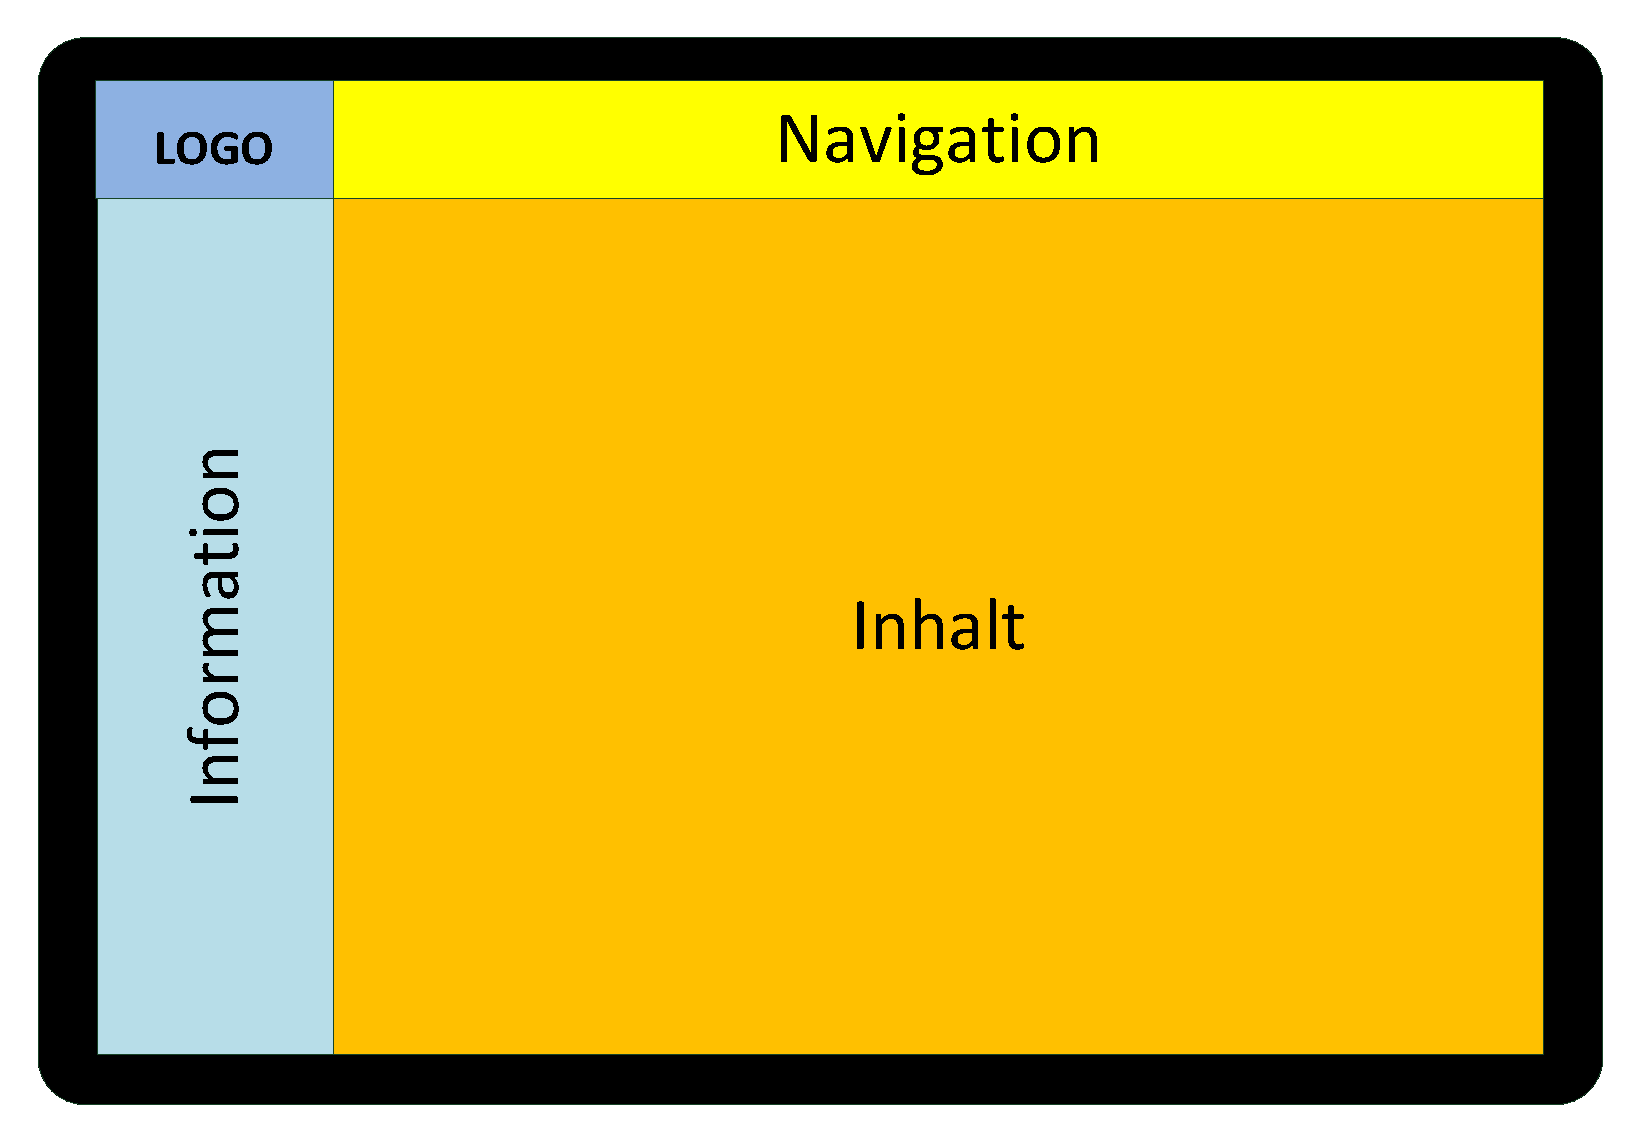
\includegraphics[scale=0.4]{figures/GUICareNetMobile.pdf}
	\caption{Struktur der grafischen Oberfl�che von \app}
	\label{fig:gui}
\end{figure}

Die Strukturierung und Gestaltung der grafischen Oberfl�che erfolgt mittels HTML5 und CSS3, die Funktionalit�t wird
mit JavaScript entwickelt. Gegen�ber der Entwicklung einer nativen Anwendung f�r Android ergeben sich bei der
Entwicklung mit JavaScript gewisse Schwierigkeiten. W�hrend Java eine objektorientierte Sprache ist, bei der
Typsicherheit und Kapselung von Funktionalit�t in Klassen zu den Eigenschaften geh�ren, ist JavaScript eine
Scriptsprache, die keinerlei Typsicherheit und nur bedingte Kapselungsm�glichkeiten bietet. Ein wichtiger Unterschied
ist, dass Java vor der Ausf�hrung zun�chst kompiliert, d.h. in eine maschinenverst�ndliche Zwischensprache �bersetzt
werden muss, w�hrend JavaScript direkt vom Browser interpretiert werden kann. Dies impliziert, dass JavaScript-Code,
selbst wenn er bereits auf einer Webseite ausgef�hrt wird, dem Nutzer im Klartext zur Verf�gung steht, w�hrend der
Java-Code nur bedingt und durch aufwendige Verfahren wieder dekompiliert und somit im Klartext verf�gbar gemacht werden
kann. Dieser Eigenschaft muss sich ein Entwickler besonders im Bezug auf im Quellcode vermerkte sicherheitsrelevante
Informationen bewusst sein.\\
W�hrend der Entwicklung kann vor allem die fehlende M�glichkeit der Kapselung problematisch werden. Abbildung
\ref{fig:vergleichJavaJS} zeigt Beispielimplementierungen in Java und JavaScript. Links wurde eine Klasse erstellt, die
Methoden und Variablen kapselt. Wird eine Variable au�erhalb einer Methode definiert (Abbildung
\ref{fig:vergleichJavaJS}: \textit{ersteVariableJava}), ist diese in der gesamten Klasse verf�gbar. Ist die Variable
als \textit{public} gekennzeichnet, kann auf sie �ber \textit{Klassenname.variablenName} zugegriffen werden.
Wird sie als \textit{private} deklariert, ist sie nur innerhalb der Klasse verf�gbar. Das gleiche gilt f�r Methoden.
Wird eine Variable innerhalb einer Methode definiert (Abbildung \ref{fig:vergleichJavaJS}: \textit{zweiteVariable}),
kann auch nur innerhalb dieser Methode auf die Variable zugegriffen werden.\\

\begin{figure}
	\centering
	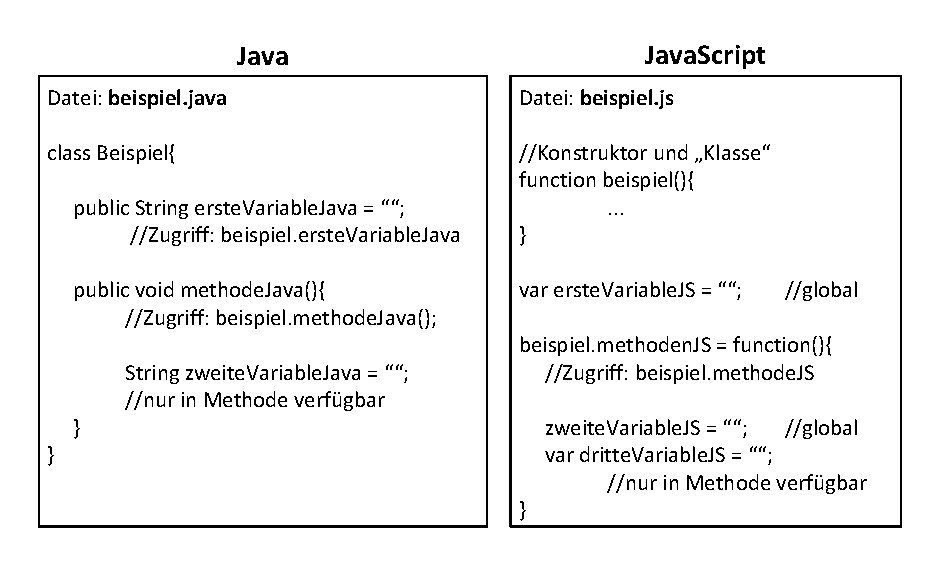
\includegraphics[width=\textwidth]{figures/VergleichJavaJavaScript.pdf}
	\caption{Vergleich zweier Beispielimplementierungen von Java und JavaScript}
	\label{fig:vergleichJavaJS}
\end{figure}

In JavaScript sind grunds�tzlich alle Methoden global verf�gbar. Die Verf�gbarkeit beschr�nkt sich hier nicht auf eine
Klasse oder Datei, sondern auf eine einmal deklarierte Methode kann von allen anderen JavaScript- und HTML-Dateien, die
gleichzeitig mit dieser Datei vom Browser geladen wurden, zugegriffen werden. Eine Klassendefinition kann nur in sofern
erfolgen, dass einem Methodennamen der Name einer anderen vorher definierten Methode vorangestellt wird (Abbildung
\ref{fig:vergleichJavaJS}: \textit{beispiel.methodeJS()}). Hiermit wird es m�glich, einen Namensraum zu definieren,
um Methoden einem bestimmten Kontext (hier: \textit{beispiel}) zuzuordnen. Wird allerdings an anderer Stelle im
geladenen JavaScript-Code die selbe Kontext-Methodennamen-Kombination verwendet, kann der Interpreter, der Browser,
keine eindeutige Zuordnung des Namens zu ausf�hrbarem Quellcode mehr herstellen und es wird nichts ausgef�hrt.\\
Ebenso verh�lt es sich mit Variablen. Wird eine Variable mit dem Zusatz \textit{var} au�erhalb einer Methode definiert,
ist sie global verf�gbar. Das gleiche gilt, wenn eine Variable ganz ohne Zusatz (Abbildung
\ref{fig:vergleichJavaJS}: \textit{zweiteVariableJS}) definiert wird. Nur wenn eine Variable innerhalb einer Methode mit
dem Zusatz \textit{var} erstellt wird, kann sie nur innerhalb der Methode verwendet werden. Dieser Umstand kann zu
massiven Problemen f�hren. Vergisst ein Entwickler beispielsweise nur ein einziges Mal den Zusatz \textit{var} bei der
Definition einer Laufvariable in einer Schleife (h�ufig mit dem Namen \textit{i}), wird diese nun global geltende
Variable alle anderen Schleifen, die ebenfalls die Laufvariable \textit{i} verwenden, beeinflussen. Da dies kein
syntaktischer, sondern ein semantischer Fehler ist, kann dieser nicht von automatisierten Fehlerfindungswerkzeugen
entdeckt werden und es beginnt die sprichw�rtliche Suche nach der Nadel im Heuhaufen. Derartige Umst�nde k�nnen sehr
viel Zeit kosten.\\

Einzelne Plug-Ins sollen die in Abbildung \ref{fig:gui} gezeigte Struktur nutzen, um Inhalte darzustellen. Damit dies
m�glich ist, m�ssen die einzelnen Bereiche, welche als HTML-DIV-Elemente erstellt wurden, eindeutig durch \acs{id}s
gekennzeichnet werden. Da es in JavaScript nicht, wie in Java, m�glich ist, Konstanten zu definieren, wurden in einer
separaten JavaScript-Datei \textit{CONSTANTS.js} alle \acs{id}s in Form von Variablen hinterlegt, welche den
DIV-Elementen zugewiesen wurden. Der Nachteil von Variablen ist, dass diese w�hrend der Laufzeit aus den Plug-Ins heraus
ver�ndert werden k�nnen. Aus diesem Grund muss die Konvention eingehalten werden, zentral definierte Variablen nicht zu
ver�ndern, da dies Auswirkungen auf andere Plug-Ins haben k�nnte. Die Eigenschaft einer Plug-In-Architektur, dass
Plug-Ins keinen Einfluss auf die Basisanwendung haben, kann somit nicht vollst�ndig in JavaScript umgesetzt werden.
Menschliche Fehler durch Nicht-Einhaltung der Konvention bleiben m�glich.\\
Der Vorteil von zentral definierten Variablen ist, dass an einer zentralen, �bersichtlichen Stelle nachgeschaut werden
kann, wie eine \acs{id} lautet, und dass die wichtigen Strukturelemente f�r Informationen, Navigation und Inhalt zentral
referenziert werden k�nnen. Die Datei \textit{CONSTANTS.js} wird au�erdem dazu genutzt, um alle sonstigen in der
Implementierung verwendeten Zeichenketten als Variablen zu hinterlegen. Hierzu z�hlt beispielsweise die Server-Adresse
der Middleware oder alle Arten von Meldungen an einen Nutzer. Dieses Verfahren erh�ht die Wartbarkeit der Anwendung, da
�nderungen an mehrfach verwendeten Zeichenketten nicht \textit{mehrfach} umgesetzt werden m�ssen, sondern lediglich
\textit{einmal} in der zentralen Datei. Die Wahrscheinlichkeit f�r Fehler durch nicht vollst�ndig umgesetzte
Anpassungen kann so verringert werden. Dieses Vorgehen ist angelehnt an die zentrale Verwaltung von \textit{String
Ressources} bei der Entwicklung nativer Android-Anwendungen \cite{androidStringRessources}.\\

Eine Grundfunktion, welche die Basisanwendung zur Verf�gung stellt, ist ein Log-In zur Sicherung der pers�nlichen Daten
und einer Identifizierung des Nutzers. Da \app eine mobile Erweiterung von CareNet darstellt, werden keine gesonderten
Konten f�r die Nutzung der mobilen Anwendung angelegt, sondern es werden die schon existierenden Konten in CareNet
verwendet. Eine M�glichkeit w�re, alle relevanten Daten f�r einen Log-In aller m�glichen Nutzer auf dem Endger�t zu
speichern und einen lokalen Abgleich zu machen, jedoch k�nnte hierdurch ein Sicherheitsproblem entstehen. Aus diesem
Grund wird bei einem Log-In eine Anfrage an CareNet gesendet, ob die eingegebenen Daten korrekt sind. Ben�tigt werden
beim Login der Mandant, der Benutzername und das Passwort. Der Log-In erfolgt in der mobilen Anwendung �ber ein
separates Fenster (eigenst�ndige HTML-Datei) in Form eines Dialogs. Erst wenn von CareNet eine Best�tigung der
Log-In-Daten erhalten wurde, wird die entsprechende HTML-Datei zur Anzeige von Inhalten geladen. Dies verhindert, dass
durch eventuelle Anzeigefehler einem noch nicht authentifizierten Nutzer sensible Daten angezeigt werden, die schon
im Hintergrund bereitliegen.\\

\begin{figure}
	\centering
	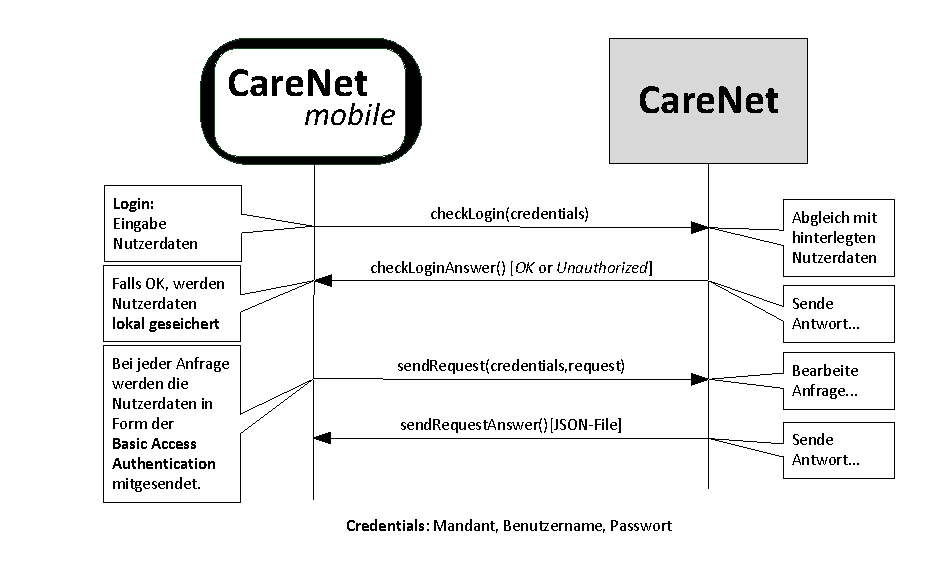
\includegraphics[width=\textwidth]{figures/AuthentifizierungCareCMviaREST.pdf}
	\caption{�berpr�fung der Benutzerdaten in \app }
	\label{fig:login}
\end{figure}

In Kapitel \ref{sec:entwurfsentscheidungen} wurde die Kommunikation von \app mit CareNet via \acs{rest} erkl�rt. Aus
dieser Kommunikation resultiert eine Besonderheit bei der Authentifizierung eines Nutzers mit einem zentralen System.
Abbildung \ref{fig:login} zeigt die notwendigen Schritte zur Authentifizierung eines Nutzers und dem anschlie�enden
Senden einer Anfrage. Da keine Sitzung aufgebaut werden kann, in der ein Nutzer dauerhaft angemeldet wird, m�ssen
die kompletten Nutzerdaten bei jeder Anfrage mitgesendet werden.\\
Meldet sich ein Nutzer in \app an, so werden zun�chst nur die eingegebenen Daten an CareNet gesendet. Als Antwort kommt
entweder der HTML-Code 200 (\textit{OK}) oder 401 (\textit{Unauthorized}). Sind die Daten korrekt (Code = 200), werden
sie im lokalen Speicher der Anwendung abgelegt, um sie f�r sp�tere Anfragen an CareNet nicht noch einmal eingeben zu
m�ssen. Hierzu kann der von HTML5 angebotene lokale Key-Value-Speicher genutzt werden. In diesem Speicher k�nnen
Zeichenketten, referenziert �ber einen Schl�ssel, permanent abgelegt werden und auch nach dem Schlie�en der hybriden
mobilen Anwendung wieder abgerufen werden. Die Nutzerdaten werden hier allerdings unverschl�sselt abgelegt. Aus
diesem Grund werden die Nutzerdaten aus dem lokalen Speicher gel�scht, sobald sich der Nutzer wieder von
\app abmeldet. Weitere Anfragen an CareNet sind so nicht mehr m�glich.\\
In Abbildung \ref{fig:login} wird die Rolle der Middleware vernachl�ssigt, da diese nicht f�r das grunds�tzliche
Kommunikationsprinzip relevant ist. Tats�chlich �bernimmt die Middleware aber einen Arbeitsschritt bei der
Kommunikation. Die Nutzerdaten werden als Zeichenkette \textit{Mandant/Benutzername:Passwort} an die Middleware
�bertragen. CareNet ben�tigt die Daten zur Authentifizierung jedoch in Form einer nach der Base Access Authentication
verschl�sselten Zeichenkette. Base Access Authentication ist \textcolor{red}{[Erl�rung Base64 nach Network security:
private communication in a public world, second edition]}. Da PHP standardisierte Methoden zur Erstellung dieser
Verschl�sselung anbietet, wurde entschieden, die Verschl�sselung in die Middleware zu verlagern.\\
Auch wenn es sich bei der Base Access Authentication namentlich um eine Verschl�sselung handelt, ist diese jedoch kein
Schutz gegen einen Zugriff auf die Daten Dritter, da das Verfahren �ffentlich bekannt ist. Im Prinzip werden die
Benutzerdaten also im Klartext von \app zu CareNet �bertragen. H�rt ein Dritter die Kommunikation ab, kann er die
Nutzerdaten auslesen und zweckentfremden. Aus diesem Grund muss die Verbindung an sich verschl�sselt werden.
Hierzu wird eine \acs{https}-Verbindung sowohl von \app zur Middleware als auch von der Middleware zu CareNet verwendet.
\textcolor{red}{[https erkl�ren mit security Buch]}.

\section{Einbinden von Plug-Ins in die Basisanwendung}

\begin{figure}
	\centering
	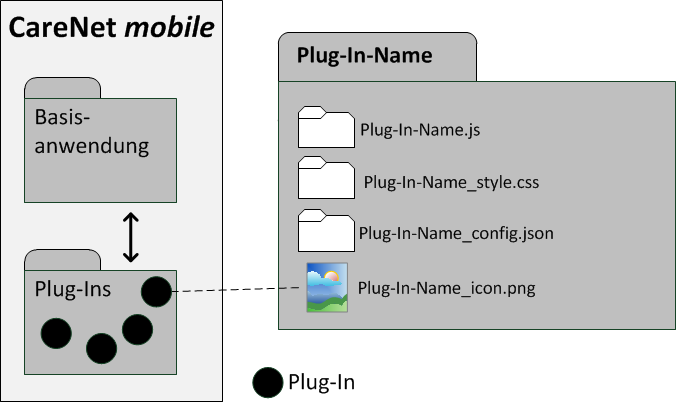
\includegraphics[scale=0.7]{figures/PluginStrukturAmbuNetMobile.png}
	\caption{Struktur eines Plug-Ins in \app}
	\label{fig:plugin}
\end{figure}

Wie in Kapitel \ref{sec:entwurfsentscheidungen} beschrieben, wird \app auf Basis einer Plug-In-Architektur entwickelt.
Die eigentliche Funktionalit�t, um die Anwendung produktiv einsetzen zu k�nnen, soll ausschlie�lich �ber Plug-Ins
hinzugef�gt werden. Diese sind prinzipiell gekapselte Programmst�cke, die bestimmte Funktionen bereitstellen. Plug-Ins
sollen der Basisanwendung leicht hinzugef�gt und wieder entfernt werden k�nnen.\\
Plug-Ins werden in \app in Form eines Ordners zum Zeitpunkt der Entwicklung eingebunden, bevor die Anwendung zur
Installation auf dem Tablet-PC generiert wird. Ein Einbinden von Plug-Ins zur Laufzeit ist somit nicht m�glich. Um eine
unbegrenzte Anzahl Plug-Ins �ber ein generisches Verfahren einbinden zu k�nnen, muss eine einheitliche Struktur gegeben
sein.  Abbildung \ref{fig:plugin} zeigt die Struktur eines Plug-Ins. Es besteht aus einer Menge von Dateien, die in
einem Ordner zusammengefasst werden. Der Ordner muss den Namen des Plug-Ins tragen und die darin enthaltenen Dateien
m�ssen der Namenskonventionen folgen, dass sie jeweils den Namen des Plug-Ins enthalten und ein beschreibendes Stichwort
f�r den Inhalt der Datei. Zwar k�nnte auch schon die Dateiendung als Indikator f�r den Inhalt dienen, jedoch wird es
durch den beschreibenden Zusatz noch eindeutiger.\\
Jedes Plug-In muss die in Abbildung \ref{fig:gui} gezeigte Struktur der Anwendung nutzen und die einzelnen Div-Elemente
�ber die in Variablen abgelegten \acs{id}s ansteuern. Um nicht bei jeder Ver�nderung eine neue HTML-Datei laden zu
m�ssen, wird der Inhalt der Div-Elemente dynamisch angepasst. Hierzu ist JavaScript notwendig, folglich muss ein Plug-In
eine JavaScript-Datei enthalten (\textit{Plug-In-Name.js}), die sowohl die Methoden zum Aufbau der grafischen Oberfl�che
als auch die Anwendungslogik enth�lt. Wichtig f�r die grafische Darstellung von \acs{html}-Elementen sind \ac{css}. Sie
wird dazu verwendet, wiederverwendbare Formatierungen zu hinterlegen, die den \acs{html}-Elementen zugewiesen werden
k�nnen. Diese m�ssen, wie JavaScript auch, in einer separaten Datei zusammengefasst werden
(\textit{Plug-In-Name\_style.css}).\\
Die Basisanwendung soll keinerlei Abh�ngigkeiten zu den Plug-Ins haben, jedoch verwenden Plug-Ins von der Basisanwendung
bereitgestellte Methoden. Au�erdem k�nnen Abh�ngigkeiten der Plug-Ins untereinander bestehen. Sind notwendige Methoden
nicht verf�gbar oder wurden diese ver�ndert (beispielsweise die Methodensignatur), kann dies dazu f�hren, dass ein
Plug-In nicht mehr funktioniert. Um die fehlenden Abh�ngigkeiten nicht erst zu entdecken, w�hrend der Nutzer eine nicht
verf�gbare Funktion versucht zu verwenden, m�ssen Abh�ngigkeiten in einer Konfigurationsdatei beschrieben werden. Die
Datei \textit{Plug-In-Name\_config.json} enth�lt eine Liste aller Plug-Ins sowie deren Versionsnummer, die ein Plug-In
ben�tigt, um grunds�tzlich funktionieren zu k�nnen. Au�erdem enth�lt die Datei die Versionsnummer des Plug-Ins selbst,
um eventuelle �nderungen anzuzeigen. Werden nun Plug-Ins beim �ffnen der Anwendung geladen, kann zun�chst �berpr�ft
werden, ob alle notwendigen Abh�ngigkeiten aufgel�st werden k�nnen. Ist dies nicht der Fall, wird ein Plug-In nicht
geladen und der Nutzer bekommt einen Hinweis angezeigt. Neben den Abh�ngigkeiten zu anderen Plug-Ins k�nnen au�erdem
Abh�ngigkeiten zu JavaScript-Bibliotheken wie jQuery mobile oder PhoneGap bestehen. Um hier Redundanzen zu vermeiden,
die entstehen, wenn jedes Plug-In diese Bibliotheken selbst einbindet, k�nnen auch diese in der Konfigurationsdatei
angegeben werden. So wird der ben�tigte Speicherplatz der Anwendung m�glichst gering gehalten.\\

\begin{figure}
	\centering
	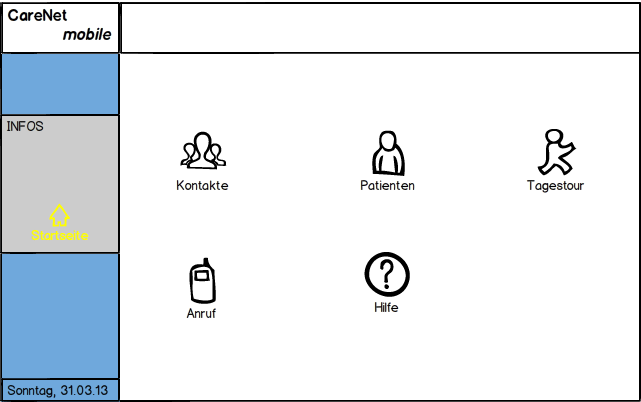
\includegraphics[scale=0.5]{figures/Startseite.png}
	\caption{�bersicht der verwendbaren der Plug-Ins}
	\label{fig:pluginView}
\end{figure}

Die Basisanwendung soll auf einer Seite einen �berblick �ber die verwendbaren Plug-Ins anbieten. Hier gibt es
verschiedene M�glichkeiten der Darstellung. Es k�nnte beispielsweise eine Liste mit den Namen aller Plug-Ins angezeigt
werden, es k�nnte eine Repr�sentation durch Symbole erfolgen oder eine Kombination aus Symbolen und Namen verwendet
werden. Da \app auf einem Tablet-PC verwendet wird, der durch Ber�hrung gesteuert wird, ist eine Liste keine gute
Alternative, da die Bedienung nicht so Pr�zise erfolgen kann wie mit einer Maus an einem PC. Fehler bei der Auswahl von
Plug-Ins sind so leicht m�glich. Orientiert man sich an dem Bedienkonzept der Apps auf einem Tablet-PC, liegt die
Verwendung von Symbolen bzw. Icons nahe. Im Falle von \app entschieden, Symbole und einen Textbezeichner zu verwenden,
um Plug-Ins eindeutig zu kennzeichnen und eine intuitive Bedienung zu erm�glichen. Abbildung \ref{fig:pluginView} zeigt
eine exemplarische Darstellung von f�nf Plug-Ins. Da die Anzahl verwendbarer Plug-Ins unbegrenzt sein soll, werden
jeweils drei Symbole pro Reihe angezeigt und diese nach unten hin erweitert. M�ssen mehr Plug-Ins angezeigt werden, als
Platz auf dem Bildschirm zu Verf�gung steht, kann der Bereich f�r den Inhalt nach unten gescrollt werden. Jedes Plug-In
muss ein eigenes Icon mit dem Namen \textit{Plug-In-Name\_icon.png} bereitstellen.\\
Zur Zeit der Abgabe dieser Arbeit war es leider noch nicht m�glich, JavaScript- und CSS-Dateien zur Laufzeit
einzubinden. Es muss jede Datei im Plug-In-Ordner manuell in der zentralen HTML-Datei eingebunden werden. Dies
verursacht zus�tzlichen Aufwand, jedoch konnte keine andere L�sung gefunden werden. Au�erdem muss der Name jedes
Plug-Ins in einer Konfigurationsdatei der Basisanwendung hinterlegt werden, denn es werden nur die Plug-Ins eingebunden,
die hier aufgelistet wurden. Ein Nachteil der manuellen Einbindung \textit{einer} JavaScript-Datei ist, dass nicht
einfach eine Menge von Dateien hinterlegt werden kann, die automatisch verwendet werden. W�re dies m�glich, k�nnte die
Anwendungslogik eines Plug-Ins auf mehrere JavaScript-Dateien aufgeteilt werden. Wird nur eine Datei eingebunden, muss
jeglicher JavaScript-Code in dieser Datei zusammengefasst werden, was die �bersichtlichkeit w�hrend der Entwicklung
hindert, da diese Datei mehrere tausend Zeilen Code enthalten kann.\\

\begin{figure}
	\centering
	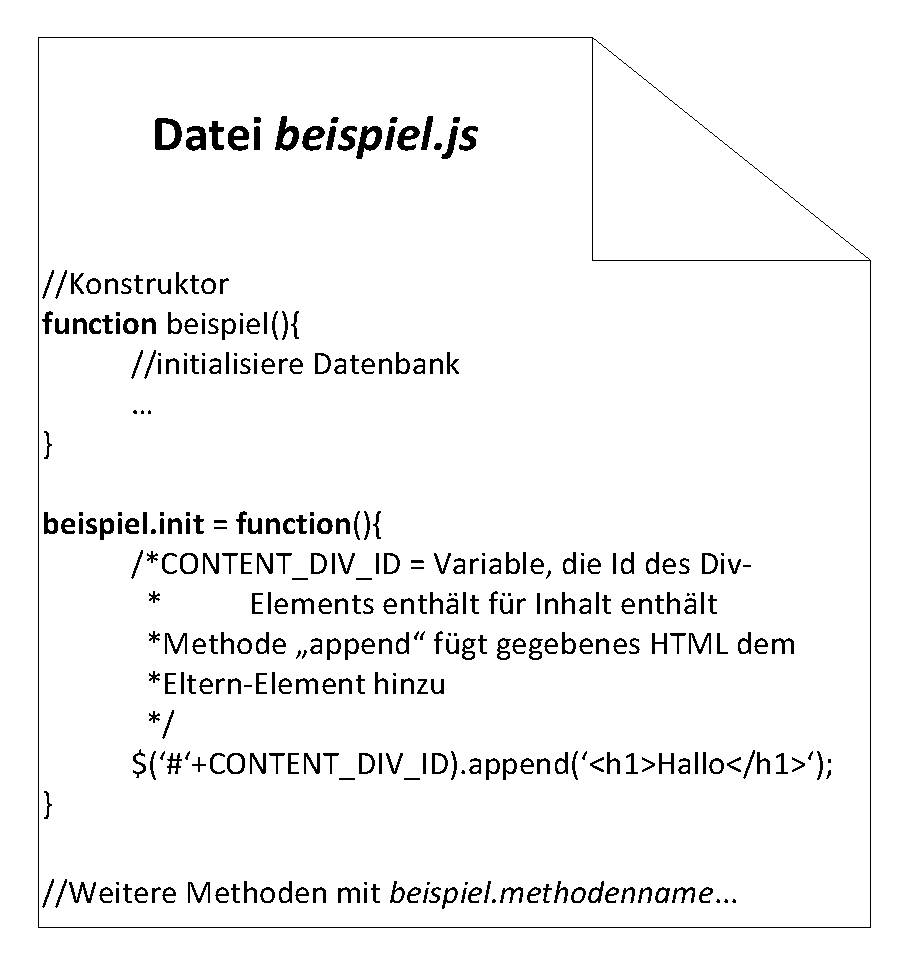
\includegraphics[scale=0.6]{figures/aufbauJsDatei.pdf}
	\caption{Grundstruktur einer Plug-In-JavaScript-Datei}
	\label{fig:pluginJsFile}
\end{figure}

Die Benutzung von \app soll auch ohne eine Internetverbindung m�glich sein, wenn vorher alle relevanten Daten auf den
Tablet-PC geladen wurden. Hierzu wird eine lokale Datenbank von der Basisanwendung bereitgestellt. Die Einzelnen
Plug-Ins k�nnen �ber vordefinierte Methoden eigene Tabellen anlegen, um Plug-In spezifische Informationen
abzuspeichern. Damit es beim ersten �ffnen eines Plug-Ins zu keiner gr��eren Verz�gerung wegen des Anlegens ben�tigter
Tabellen kommt, ist eine Funktion w�nschenswert, mit der Plug-Ins Vorg�nge ansto�en k�nnen, die schon vor dem ersten
�ffnen ausgef�hrt werden. Um dies zu erm�glichen, muss die JavaScript-Datei die in Abbildung \ref{fig:pluginJsFile}
gezeigten Methoden implementieren.\\
Ben�tigt wird zun�chst ein Konstruktor, der nach dem Plug-In benannt wurde. Dieser wird aufgerufen, sobalb ein Plug-In
zur Anzeige auf der �bersicht geladen und festgestellt wurde, dass all Abh�ngigkeiten erf�llt sind. Hier k�nnen
beispielsweise Tabellen einer Datenbank initialisiert werden. Neben einem Konstruktor wird eine Methode zur
Initialisierung der Anwendung ben�tigt. Diese wird aufgerufen, sobald ein Nutzer ein Plug-In �ffnet. In dieser Methode
muss die Anzeige der App in den Bereichen Navigation, Information und Inhalt angepasst werden. Beispielsweise k�nnte ein
Button in die Navigationsleiste gesetzt werden oder, wie in Abbildung \ref{fig:pluginJsFile} gezeigt, dem Inhalts-Div
der Schriftzug "`Hallo"' in dem HTML-Gr��enelement "`<h1>"' hinzugef�gt werden. W�rde die Plug-In-Struktur in Java
implementiert, k�nnte die Methode \textit{init()} in ein Interface gefasst werden, welches jedes Plug-in implementieren
muss. Auch ein Konstruktor w�re gegeben. Dies w�re eine bessere Variante, da so sichergestellt werden kann, dass ein
Programmierer die Methoden implementiert (alle Methoden eines verwendeten Interfaces m�ssen in Java implementiert
werden). In JavaScript kann die Anforderung nur �ber Konventionen eingefordert werden, was zu menschlichen Fehlern durch
Vergessen der Methoden f�hren kann.\\
�hnlich wie bei der Namensgebung der Dateien m�ssen auch innerhalb der Dateien Konventionen eingehalten werden. Um zu
verhindern, dass Methoden mit gleichen Namen oder CSS-Klassen mit gleichen Namen in verschiedenen Plug-Ins implementiert
werden, die sich dann gegenseitig st�ren, muss jede Methode mit dem Namen des Plug-Ins beginnen
(\textit{Plug-In-Name.methode}), ebenso wie jede CSS-Klasse, jedoch hier ohne Punkt (\textit{Plug-In-NameKlassenname}).
Auch jede global verwendete Variable muss den Plug-In-Namen vorangestellt bekommen, um Konflikte zu vermeiden. Eine
Nicht-Einhaltung der Konventionen kann zu einer v�lligen Funkionsst�rung der Anwendung f�hren.


\section{Das Plug-In "`Kontakte"'}
F�r alle Plug-Ins feste Beschreibungsstruktur:
\begin{itemize}
  \item Begr�ndung f�r Plug-In (aus welchen Anforderungen geht Plug-In hervor)
  \item Aufbau/Navigationsstruktur
  \item Zentrale Frage, die beantwortet werden muss: Welche Funktionalit�t geht aus welcher
  Anforderung hervor?
\end{itemize}

\ldots

\section{Das Plug-In "`Touren"'}
\ldots

%% ==================
\chapter{Evaluation}
\label{ch:Evaluation}
%% ==================

Im folgenden Kapitel wird die bisher entwickelte Anwendung zur Unterst�tzung der Dokumentation von delegierten
�rztlichen T�tigkeiten evaluiert. In Abschnitt \ref{sec:iso25k} wird \app zun�chst an Qualit�tskriterien der
\acs{iso}/\acs{iec} 25000 gemessen, die auf die Software-Produktqualit�t abzielt. In Abschnitt
\ref{sec:evalEndnutzer} wird das Ergebnis einer Anforderungsevaluation im Rahmen einer Schulung von Angeh�rigen der
Alten- und Krankenpflegeberufe vorgestellt.

\section{Evaluation der technischen Umsetzung der mobilen Anwendung}
\label{sec:iso25k}

Zur Evaluation der entwickelten Anwendung wird auf den von der \acl{iso} (\acs{iso}) und der \acl{iec} (\acs{iec})
entwickelten Standard 25000 zur�ckgegriffen, der den Namen "Software product Quality Requirements and Evaluation
(SQuaRE)" tr�gt \cite{iso25000}. Der Standard ersetzt die beiden �lteren Standards ISO/IEC 14598 (Software Product
Evaluation) und ISO/IEC 9126 (Software Product Quality), da diese ohnehin komplement�ren Standards die gleichen
normativen und funktionellen Wurzeln bildeten, jedoch Inkonsistenzen in den vorgeschlagenen Lebenszyklen auftraten. Der
Standard ISO/IEC 25000 soll Entwicklern, K�ufern und unabh�ngigen Gutachtern von Software-Produkten eine Menge von
Kriterien zur Bewertung von Software in verschiedenen Entwicklungsphasen bieten. Von der Anforderungsanalyse �ber die
Implementierung bis hin zum fertigen Software-Produkt werden Methoden vorgeschlagen, mit denen eine Koordination
zwischen Messung und Evaluation von definierten Charakteristika vorgenommen werden kann. Definiert wird ein
Software-Produkt Lebenszyklus, in welchem die Software-Produkqualit�t in drei Phasen erfasst wird. Diese sind die
\textit{Qualit�t w�hrend der Benutzung} (Quality in Use), die \textit{externe Qualit�t} (external Quality) und die
\textit{interne Qualit�t} (internal Quality). Erstere beschreibt die Anforderungen an die Software aus Sicht des
Endnutzers beim finalen Endprodukt. Die externe Qualit�t wird aus den Endnutzeranforderungen abgeleitet und als Ziel f�r
die technische  Verifikation und Validierung der Sofware genutzt. Die interne Qualit�t wird wiederum zum Teil aus den
Anforderungen an die externe Qualit�t abgeleitet, definiert werden aber auch die Eigenschaften von
Software-Zwischenprodukten auf dem Weg zum Endprodukt. Die internen Qualit�tskriterien k�nnen auch auf Nebenprodukte der
Entwicklung wie die Dokumentation oder Anleitungen angewandt werden. Die Evaluation von \app erfolgt nur auf Basis der
internen und externen Qualit�tskriterien, da es w�hrend der begrenzten Bearbeitungszeit nicht m�glich war, eine
marktreife Anwendung zu entwickeln, sondern lediglich einen Prototypen. Au�erdem fehlen zu einer vollst�ndigen
Evaluation tats�chliche Endnutzer, die f�r die Beurteilung der Qualit�t w�hrend der Benutzung unerl�sslich sind.

\begin{figure}[ht]
	\centering
	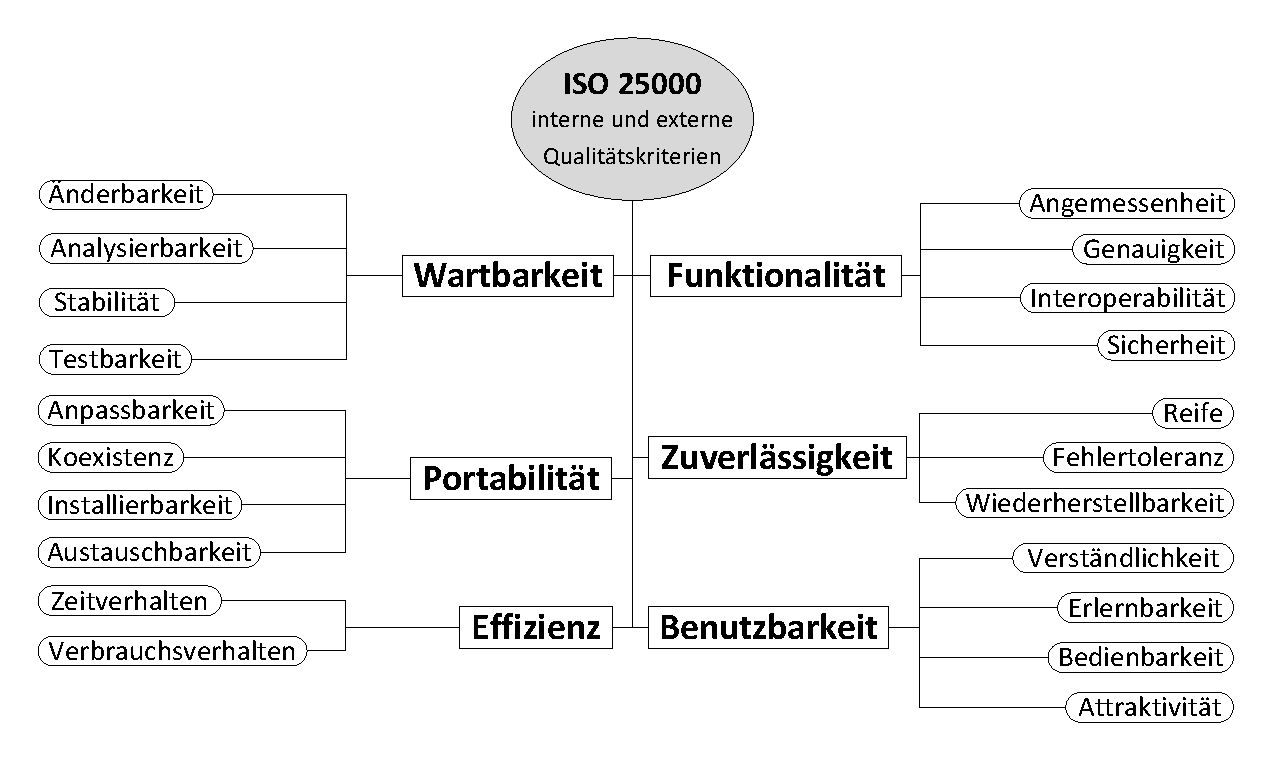
\includegraphics[width=\textwidth]{figures/iso25k.pdf}
	\caption{Interne und externe Charakteristika von Software-Produktqualit�t}
	\label{fig:iso25k}
\end{figure}

Abbildung \ref{fig:iso25k} zeigt die Charakteristika und Subcharakteristika f�r die Bewertung der internen und externen
Qualit�t. Zu jedem Charakteristikum geh�rt neben den in der Grafik gezeigten Subcharakteristika noch die Konformit�t zum
Charakteristikum selbst, jedoch macht eine Evaluation dieser Eigenschaft nur beim tats�chlichen Endprodukt Sinn. Da
dieses nicht vorhanden ist, wird die Konformit�t generell nicht betrachtet. Die folgende Auflistung gibt zu jedem der in
Abbildung \ref{fig:iso25k} gezeigten Subcharakteristika eine Einsch�tzung ab, ob und wenn ja wie dieses in \app
adressiert wurde. In kursiver Schrift ist jeweils die Definition des Subcharakteristikums gegeben. 

\Large 
\textbf{Wartbarkeit}

\normalsize

\begin{description}
	\item[�nderbarkeit] 
	\textit{"F�higkeit des Softwareprodukts, die Implementierung einer spezifizierten �nderung zu erm�glichen."} \cite[S.
	470]{balzert}
	\vspace{0.2cm}
	
	Die technischen Anforderungen an \app zielten vor allem auf eine leichte Erweiterbarkeit und �nderbarkeit wegen
	ver�nderter Rahmenbedingungen ab. Gefordert wurde ein modularer Aufbau, der in einer Plug-In-Architektur umgesetzt
	wurde. Eine leichte �nderbarkeit bzgl. Hinzuf�gen und Entfernen von Plug-Ins wurde folglich adressiert, jedoch sind
	Ver�nderungen \textit{innerhalb} eines Plug-Ins oder der Basisanwendung schwieriger umzusetzen, da durch die Verwendung
	von nur einer JavaScript-Datei pro Modul nur eine verh�ltnism��ig un�bersichtliche Quellcode-Basis zur Verf�gung
	steht. Durch ausf�hrliche Kommentierung des Quellcodes wurde versucht, die fehlende Struktur auszugleichen.
	
	\item[Analysierbarkeit]
	\textit{"F�higkeit des Softwareprodukts, M�ngel oder Ursachen von Versagen zu diagnostizieren oder �nderungsbed�rftige
	Teile zu identifizieren."} \cite[S.470]{balzert}
	\vspace{0.2cm}
	
	Die grunds�tzliche Struktur ist aufgrund seines modularen Aufbaus gut analysierbar, da die Zusammenh�nge und
	Abh�ngigkeiten �ber die Konfigurationsdateien nachvollziehbar sind. Sollen allerdings Aufrufketten von Funktionen
	verfolgt werden, muss dies in der Regel manuell gemacht werden, da hier keine Unterst�tzung durch Software-Werkzeuge
	vergleichbar beispielsweise mit der Unterst�tzung, die Eclipse \cite{eclipse} bei der Java-Entwicklung bietet,
	vorhanden ist. Eine Analyse ist zwar immer noch m�glich, jedoch ist die Gefahr gr��er, dass hierbei wegen der
	fehlenden Automatisierung Fehler passieren. Auch das Finden von Fehlern gestaltet sich schwierig, da in JavaScript
	auftretende Fehler im Programmablauf (Exceptions) h�ufig nur unzureichend dokumentiert werden.
	
	\item[Stabilit�t]
	\textit{"F�higkeit des Softwareprodukts, unerwartete Wirkungen von �nderungen der Software zu
	vermeiden."} \cite[S.470]{balzert}
	\vspace{0.2cm}
	
	Die Stabilit�t der Anwendung stand bisher nicht im Fokus der Entwicklung. Zwar wurden Instabilit�ten
	behoben, wenn sie entdeckt wurden, jedoch konnte aufgrund des zeitlichen Rahmens keine ausf�hrliche Analyse bez�glich
	m�glicher instabiler Abl�ufe durchgef�hrt werden.
	
	\item[Testbarkeit] 
	\textit{"F�higkeit des Softwareprodukts, Standards oder Konventionen bezogen auf die Wartbarkeit einzuhalten."}
	 \cite[S.470]{balzert}
	\vspace{0.2cm}
	
	\app besteht aufgrund seines hybriden Charakters aus einer Menge verschiedener Technologien. Der
	native Container besteht aus der jeweils zugrunde liegenden Programmiersprache, w�hrend die haupts�chliche
	Funktionalit�t mit JavaScript implementiert wird, die Darstellung aber vollst�ndig �ber HTML und CSS l�uft. Au�erdem bestehen
	Abh�ngigkeiten zu Bibliotheken wie jQuery, jQuery mobile und PhoneGap. Theoretisch k�nnen in allen Elementen Fehler
	auftreten, was eine komplette, im Idealfall automatisierte �berpr�fung sehr schwierig macht. Zwar gibt es
	JavaScript Test-Frameworks wie Jasmine \cite{jasmine} oder QUnit (f�r jQuery) \cite{qunit}, jedoch k�nnen hiermit
	haupts�chlich Fehler im eigenen Quellcode entdeckt werden. Fehler in den extern entwickelten Bibliotheken sind so nur
	schwer zu identifizieren. Bisher wurden aus Zeitgr�nden keine automatischen Tests implementiert. Die �berpr�fung der
	grafischen Oberfl�che bestehend aus HTML und CSS, die einen signifikanten Anteil der Entwicklungszeit beansprucht hat,
	kann ohnehin nur manuell durch Blickpr�fung erfolgen. Die Pr�fbarkeit von \app ist daher als schwierig einzustufen.
\end{description}

\Large 
\textbf{Portabilit�t}

\normalsize
\begin{description}
	\item[Anpassbarkeit] 
	\textit{"F�higkeit des Softwareprodukts, die Software an verschiedene, festgelegte Umgebungen anzupassen, wobei nur
	Aktionen oder Mittel eingesetzt werden, die f�r diesen Zweck f�r die betrachtete Software vorgesehen sind."} \cite[S.
	470]{balzert}
	\vspace{0.2cm}	
	
	Die Anpassbarkeit bezieht sich bei \app vor allem auf die M�glichkeit, die Anwendung auf verschiedenen Plattformen
	(Android, iOS, Windows Phone etc.) bereitzustellen. Durch die Verwendung von PhoneGap wurde diese Art der
	Anpassbarkeit implizit mit in die Architektur aufgenommen. Dadurch, dass die Funktionalit�t von \app ausschlie�lich
	�ber JavaScript realisiert wurde, was zwischen den Plattformen portierbar ist, wurde nicht nur zum Entwurfszeitpunkt,
	sondern auch w�hrend der Implementierung ein besonderes Augenmerk auf die Erhaltung der von PhoneGap erm�glichten
	Anpassbarkeit an verschiedene Plattformen gelegt.
		
	\item[Koexistenz] 
	\textit{"F�higkeit des Softwareprodukts, mit anderen unabh�ngigen Softwareprodukten in einer gemeinsamen Umgebung
	gemeinsame Ressourcen zu teilen."} \cite[S. 470]{balzert}
	\vspace{0.2cm}
		
	Da \app gekapselt als Anwendung f�r eine jeweilige Plattform bereitgestellt wird, ist es problemlos	mit anderen
	Anwendungen auf einer Plattform kombinierbar. Auch k�nnten verschiedene Versionen der gleichen Anwendung auf dem
	Endger�t installiert sein, wenn verschiedene Signaturen der Anwendungen verwendet werden.
	
	\item[Installierbarkeit] 
	\textit{"F�higkeit des Softwareprodukts, in einer festgelegten Umgebung installiert zu werden."} \cite[S. 470]{balzert}
	\vspace{0.2cm}
	
	Zur Installation werden die von der jeweiligen Plattform unterst�tzen Verfahren verwendet, die in der Regel einfach
	und intuitiv sind, da sie f�r eine breite Masse von Nutzern verwendbar sein m�ssen. Da \app aber nicht f�r den Einsatz
	in der breiten Masse gedacht ist, sondern gezielt an Kunden weitergegeben wird und somit nur eine verh�ltnism��ig
	geringe Anzahl an Installationen durchgef�hrt werden wird, spielt die Installierbarkeit nur eine untergeordnete Rolle.
		
	\item[Austauschbarkeit] 
	\textit{"F�higkeit des Softwareprodukts, diese Software anstelle einer spezifizierten anderen in der Umgebung jener
	Software f�r denselben Zweck zu verwenden."} \cite[S. 470]{balzert}
	\vspace{0.2cm}
	
	Die Frage der Austauschbarkeit stellt sich im Kontext der Dokumentation delegierter �rztlicher T�tigkeiten kaum, da es
	bisher keine mobilen Software-Systeme f�r diesen Anwendungsbereich gibt. Grunds�tzlich muss aber angemerkt werden, dass
	die Einf�hrung von \app vor allem an die Existenz von CareNet gebunden ist. Ist CareNet vorhanden, gen�gt das Setzen
	der entsprechenden Adresse des Servers. Es m�sste also eher die Austauschbarkeit von CareNet betrachtet werden als die
	der mobilen Erweiterung.
\end{description}

\Large 
\textbf{Effizienz}

\normalsize
\begin{description}
	\item[Zeitverhalten]
	\textit{"F�higkeit des Softwareprodukts, angemessene Antwort- und Verarbeitungszeiten sowie Durchsatz bei der
	Funktionsausf�hrung unter festgelegten Bedingungen sicherzustellen."} \cite[S. 469]{balzert}
	\vspace{0.2cm}
	
	Bei \app handelt es sich nicht um eine Anwendung, bei der das Zeitverhalten ein entscheidender
	Faktor ist. Zwar soll durch den Einsatz der Anwendung Zeit gespart werden, jedoch kommt es hier nicht auf
	Millisekunden an. Die einzige zeitliche Limitierung ist die Geduld des Nutzers w�hrend der Bedienung, welche je nach
	Individuum sehr unterschiedlich ausfallen kann. Solange keine sekundenlangen Verz�gerungen beim Laden von Daten oder
	Ansichten auftreten, welche bisher nicht festgestellt werden konnten, muss das Zeitverhalten nicht n�her betrachtet
	werden.	
	
	\item[Verbrauchsverhalten] 
	\textit{"F�higkeit des Softwareprodukts, eine angemessene Anzahl und angemessene Typen von Ressourcen zu verwenden,
	wenn die Software ihre Funktionen unter festgelegten Bedingungen ausf�hrt."} \cite[S. 469]{balzert}
	\vspace{0.2cm}
	
	Die bisher betrachteten Tablet-PCs, welche f�r den Einsatz von \app in Frage kommen, sind
	in der Regel mit Ressourcen f�r die Nutzung von Multimediainhalten ausgestattet. Aufgrund dessen, dass zur
	Dokumentation von delegierten �rztlichen Leistungen lediglich einige Datenbankoperationen, die Anzeige von
	HTML-Inhalten und einige Animationen ben�tigt werden, sollten die Ressourcen der Zielger�te ausreichend sein. Da der
	Speicher der Ger�te im Gigabyte-Bereich (1 Gigabyte = 1024 Megabyte) liegt und die Anwendung zum Zeitpunkt der Abgabe
	weniger als 2 Megabyte gro� war, muss dem Verbrauchsverhalten keine besondere Aufmerksamkeit geschenkt werden.
\end{description}

\Large 
\textbf{Funktionalit�t}

\normalsize
\begin{description}
	\item[Angemessenheit] 
	\textit{"F�higkeit des Softwareprodukts, f�r spezifizierte Aufgaben und Benutzerziele geeignete Funktionen
	bereitzustellen."} \cite[S. 468]{balzert} 
	\vspace{0.2cm}
	
	Im Vergleich mit den Anforderungen ist die bisher implementierte Funktionalit�t zwar eine gute Basis, jedoch
	fehlen noch wichtige Funktionalit�ten wie das Hinzuf�gen durchgef�hrter T�tigkeiten vor Ort beim Klienten oder eine
	vollst�ndige Klienteninformation. Aus diesem Grund ist die Funktionalit�t von \app noch nicht als angemessen anzusehen.	
	
	\item[Genauigkeit]
	\textit{"F�higkeit des Softwareprodukts, die richtigen oder vereinbarten Ergebnisse oder Wirkungen mit der
	ben�tigten Genauigkeit bereitzustellen."} \cite[S. 468]{balzert}
	\vspace{0.2cm}
	
	Da noch einige Anforderungen offen sind, die f�r einen produktiven Einsatz der Software notwendig sind, kann zum
	jetzigen Zeitpunkt die Genauigkeit der Anwendung nicht abschlie�end �berpr�ft werden.	
	
	\item[Interoperabilit�t] 
	\textit{"F�higkeit des Softwareprodukts, mit einem oder mehreren vorgegebenen Systemen zusammenzuwirken."} \cite[S.
	468]{balzert}
	\vspace{0.2cm}
	
	\app wurde daf�r entwickelt, Daten von CareNet abzurufen, ver�nderbar zu machen und diese zur�ckzusenden. Zwar wird
	eine allgemeine \acs{rest}-Schnittstelle verwendet, jedoch ist die Behandlung der abgefragten Daten stark an das
	Datenmodell von CareNet angepasst. \app kann also nicht ohne Weiteres mit einem anders aufgebauten Basissystem
	verwendet werden, sondern ist an CareNet gebunden. Es ist jedoch m�glich, �ber eine Konfigurationsdatei
	verschiedene Instanzen von CareNet anzusteuern (�ber die �nderung der URL zum Server). Allerdings ist eine Erweiterung
	auf andere Produkte der nubedian GmbH denkbar (vgl. \cite{nubedian}), da diese ein �hnliches Datenmodell und die
	gleiche Schnittstelle verwenden. Eventuell w�rde hierzu die Entwicklung weiterer Plug-Ins notwendig.
	
	
	\item[Sicherheit] 
	\textit{"F�higkeit des Softwareprodukts, Informationen und Daten so zu sch�tzen, dass nicht autorisierte
	Personen oder Systeme sie nicht lesen oder ver�ndern k�nnen, und autorisierten Personen oder Systemen der
	Zugriff nicht verweigert wird."} \cite[S. 468]{balzert}
	\vspace{0.2cm}
	
	Die Sicherheit in \app muss vor allem f�r die verwendeten pers�nlichen Daten hergestellt werden. Dies
	wird lokal auf dem Endger�t �ber einen Log-In-Mechanismus realisiert, mit dem sichergestellt wird, dass nur
	autorisierte Personen Zugriff auf die Daten von Klienten und sonstigen Kontakten bekommen. Sobald die Anwendung
	verlassen wird, sie aber trotzdem noch im Hintergrund l�uft und wieder aufgerufen werden kann, werden die Nutzerdaten
	aus dem lokalen Speicher entfernt, um nicht einem Dritten, der das Endger�t in die H�nde bekommt, einen Zugang �ber die
	hinterlegten Daten zu erm�glichen. Dadurch, dass \app vom Betriebssystem einen eigenen Speicherbereich zugewiesen
	bekommt, ist ein Zugriff auf gespeicherte Inhalte von anderen Anwendungen aus nicht m�glich. Die �bertragung der Daten
	zu CareNet wird �ber eine \acs{https}-Verbindung gesichert.	
	
\end{description}

\Large 
\textbf{Zuverl�ssigkeit}

\normalsize
\begin{description}

	\item[Reife] 
	\textit{"F�higkeit des Softwareprodukts, trotz Fehlzust�nden in der Software nicht zu versagen."} \cite[S.
	468]{balzert}
	\vspace{0.2cm}
	
	Bis zum Ende der Bearbeitungszeit dieser Master-Arbeit konnte lediglich ein Prototyp einer mobilen
	Anwendung zur Dokumentation �rztlicher Leistungen entwickelt werden. Aus diesem Grund ist die Anwendung noch einige
	Entwicklungs- und Testschritte von einer marktreifen Anwendung entfernt, die mit einem breiten Spektrum von
	Fehlzust�nden umgehen kann.
	 
	\item[Fehlertoleranz] 
	\textit{"F�higkeit des Softwareprodukts, ein spezifiziertes Leistungsniveau bei Software-Fehlern oder
	Nicht-Einhaltung ihrer spezifizierten Schnittstelle zu bewahren."} \cite[S.	468]{balzert}
	\vspace{0.2cm}
	
	Zur Implementierung einer Fehlertoleranz wurden in erster Linie die von den JavaScript-Frameworks
	gegebenen Mechanismen benutzt. Beispielsweise werden Datenbankanfragen in Transaktionen gekapselt, damit eine direkte
	Fehlerbehandlung erfolgen kann, wenn eine Anfrage fehlschl�gt. Auch bei \acs{ajax}-Anfragen an CareNet wird jeweils
	�berpr�ft, ob die Anfrage erfolgreich war und wenn nicht, werden entsprechende Ma�nahmen eingeleitet.\\
	Um sicherzustellen, dass Daten an CareNet vollst�ndig �bermittelt werden, wird jedes Element (z.B. ein Messwert oder
	ein Dossier) einzeln �bertragen, um bei einem Fehler genau zu wissen, welche Operationen noch einmal ausgef�hrt werden
	muss. Die Fehlertoleranz ist allerdings noch nicht f�r alle m�glichen Anwendungsf�lle implementiert. Es besteht also
	noch Nachbesserungsbedarf.
	
	\item[Wiederherstellbarkeit] 
	\textit{"F�higkeit des Softwareprodukts, bei einem Versagen ein spezifiziertes Leistungsniveau wiederherzustellen und
	die direkt betroffenen Daten wiederzugewinnen."} \cite[S. 468]{balzert}
	\vspace{0.2cm}
	
	St�rzt die Anwendung oder das gesamte Endger�t ab, sind nicht gleich alle Daten verloren.
	Eingaben wie die Best�tigung einer Standardleistung (vgl. Kapitel \ref{sec:plugTouren}) oder die Eintragung einer
	Begr�ndung, warum eine Leistung nicht erbracht werden konnte, werden direkt bei der Eingabe in der lokalen
	Sqlite-Datenbank gespeichert. F�r Wundfotos und Messwerte muss der Speichervorgang explizit angesto�en werden.
	Da die lokale Datenbank persistent ist, k�nnen gespeicherte Daten auch nach einem Neustart des Tablet-PCs oder der
	Anwendung wiederhergestellt werden. Wird die Anwendung oder der zugeh�rige Speicherbereich allerdings gel�scht, bevor
	die Daten an CareNet �bertragen wurden, sind sie nicht wiederherstellbar.	
\end{description}

\Large 
\textbf{Benutzbarkeit}

\normalsize
\begin{description}
	\item[Verst�ndlichkeit, Erlernbarkeit, Bedienbarkeit, Attraktivit�t] Die Benutzbarkeit des Prototyps von \app wurde in
	einer Schulung mit einigen m�glichen Endnutzern evaluiert. Die Ergebnisse der Evaluation werden in Abschnitt
	\ref{sec:evalEndnutzer} vorgestellt.
\end{description}


\section{Evaluation von Nutzbarkeit, Funktionsumfang und Akzeptanz anhand einer Zielgruppenschulung}
\label{sec:evalEndnutzer}

Am 19.01.2013, nach etwa drei Monaten Entwicklungszeit, fand eine ganzt�gige EDV-Anwenderschulung im Rahmen der
Ausbildung zur Medizinischen Fachpflegekraft am Forschungszentrum Informatik (FZI) statt. Die sieben Teilnehmerinnen
waren ausgebildete Alten- und Krankenpflegerinnen mit mehrj�hriger Berufserfahrung. Der erste Teil des Tages wurde
vorwiegend zu Schulungszwecken genutzt, w�hrend der zweite Teil des Tages der Evaluation der zu Beginn der Arbeit auf
Basis von Literatur ermittelten Anforderungen an eine mobile Anwendung diente. Ziel des Schulungsteils der Veranstaltung
war einerseits eine grundlegende Einf�hrung in die Nutzung von CareNet, andererseits sollten die Teilnehmerinnen den
Umgang mit Tablet-PCs erlernen und f�r die hiermit gegebenen technischen M�glichkeiten begeistert werden. Im zweiten
Teil zur Evaluation wurde der Fokus auf die Ermittlung der momentanen Abl�ufe bei der Dokumentation pflegerischer
Leistungen gelegt, auftretende Probleme sollten identifiziert werden und daraus Anforderungen an die Dokumentation auf
einem Tablet-PC abgeleitet werden.\\

\subsection{Vorwissen der Teilnehmer und vorbereitende Ma�nahmen}
\label{subsec:vorwissen}

Zu Beginn der Schulung musste zun�chst der EDV-Wissensstand ermittelt werden, um festzustellen, welche Kenntnisse
vorausgesetzt werden k�nnen, ohne die Teilnehmer zu �berfordern. Ziel war es, zu keinem Zeitpunkt wegen zu schneller
Vorgehensweise Teilnehmer zu verlieren oder Langeweile durch zu langsames Vorgehen aufkommen zu lassen. Hierzu wurde im
Gespr�ch mit der Gruppe ermittelt, ob Computer �berhaupt Teil des t�glichen beruflichen und privaten Lebens seien und,
falls ja, welche Einstellung die Teilnehmer gegen�ber Computern haben. Ein Stimmungsbild bez�glich der Einstellung ist
als Grundlage einer Anwenderschulung besonders wichtig, da so fr�hzeitig generelle Kritikpunkte an sowie Widerst�nde
gegen \acs{edv} identifiziert werden k�nnen und gezielt dagegen gearbeitet werden kann. Werden versteckte Widerst�nde
nicht erkannt, kann dies den Erfolg einer Schulung gef�hrden.

Die Teilnehmer gaben an, sowohl privat als auch beruflich mit Computern zu arbeiten. Haupts�chlich w�rden das Internet
(verschiedene Browser) und Office-Anwendungen benutzt, sowie im Beruf die zur Dokumentation von T�tigkeiten verwendete
Software. Neben station�ren PCs wurde auch die Verwendung von Mobiltelefonen, Smartphones und Tablet-PCs abgefragt.
Mobiltelefone benutzten alle Teilnehmer, ein Smartphone besa�en jedoch nur zwei Teilnehmerinnen und Tablet-PCs wurden
lediglich einmal von zwei Teilnehmerinnen verwendet.

\begin{figure}[ht]
	\centering
	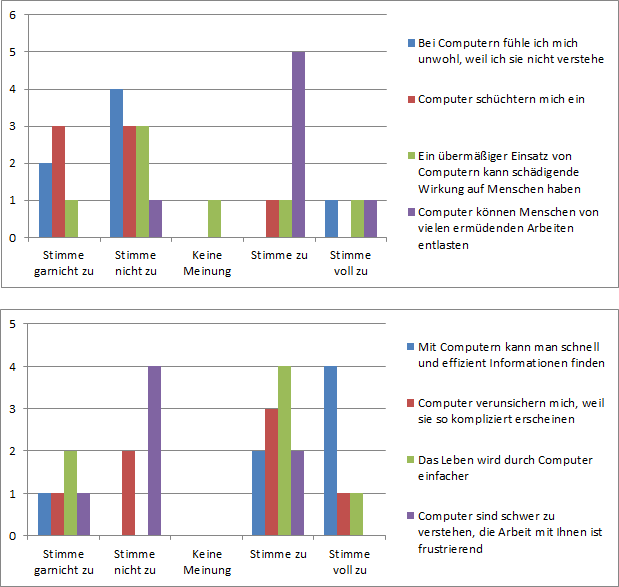
\includegraphics[scale=0.6]{figures/CASResults.png}
	\caption{Ergebnisse des Fragebogens zur Einstellung gegen�ber Computern}
	\label{fig:casResults}
\end{figure}

Zur Fundierung der in der Diskussion gewonnenen Eindr�cke wurde von den Teilnehmern ein Fragebogen zur Ermittlung der
Einstellung gegen�ber elektronischer Datenverarbeitung auf Basis des \acl{cas} (\acs{cas}) \cite{casOriginal}
ausgef�llt. Da der \acs{cas} im Jahre 1986 entwickelt wurde, als die Nutzung von Computer in Unternehmen und vereinzelt
auch in Privathaushalten gerade erst begann, konnte nur ein Teil der Fragen verwendet werden. In der Master-Arbeit von
Mathias Schmon \cite{masterMathias} wurden die Fragen bereits in einer ersten Version �bersetzt und �berarbeitet, was
als Grundlage f�r den in dieser Arbeit verwendeten Fragebogen diente. Die letztendliche Auswahl der Fragen zielte vor
allem darauf ab, wie sich die Teilnehmer bei der Arbeit mit Computern f�hlen, ob sie sie beispielsweise als Bedrohung
ansehen oder ob Computer eher als n�tzliches Hilfsmittel angesehen werden. Au�erdem wurde gefragt, ob die Teilnehmer
meinen, ein grunds�tzliches Verst�ndnis f�r die Arbeit mit Computern zu haben. Der Fragebogen wurde nach dem
Gruppengespr�ch �ber die Vorkenntnisse schriftlich und anonym von jedem Teilnehmer ausgef�llt. Der verwendete Fragebogen
ist im Anhang \ref{app:fragebogenCAS} zu finden.

Die Ergebnisse des Fragebogens sind in Abbildung \ref{fig:casResults} aufgelistet. Sechs von sieben Teilnehmern sagten
aus, dass sie sich bei der Arbeit mit Computern weder unwohl f�hlen (1), noch eingesch�chtert werden (2). Hieraus kann
geschlossen werden, dass grunds�tzlich keine Scheu gegen�ber Computern besteht. Jedoch waren sich die Teilnehmer bei der
Frage, ob Computer sie verunsichern, nicht einig (drei stimmten zu, vier nicht), was offenbart, dass trotz t�glicher
Nutzung immer noch gewisse Bedenken vorhanden sind. Dies steht in gewissem Widerspruch zu der Frage, ob Computer
verunsichernd wirken (6), da Unsicherheit h�ufig zu Unwohlsein f�hrt. Auch bei der Frage, ob ein �berm��iger Einsatz von
Computern sch�digende Wirkung haben k�nnte (3), herrschte keine Einigkeit. Obwohl vier von sieben Teilnehmern der These
nicht zustimmten, kann aus der Diversit�t der Antworten geschlossen werden, dass eine fl�chendeckende Einf�hrung von
Computern kritisch gesehen wird. Die Fragen zum Nutzen von Computern bei der Ausf�hrung der t�glichen Arbeit fielen
grunds�tzlich positiv aus. Zwar stimmten jeweils ein bzw. zwei Teilnehmerinnen den Thesen nicht zu, dass Computer
erm�dende Aufgaben �bernehmen k�nnen (4), man mit ihnen schnell Informationen finden kann (5) und sie das Leben
grunds�tzlich vereinfachen (7), jedoch l�sst sich daraus ablesen, dass Computer als Hilfsmittel und nicht als H�rde
angesehen werden. Trotz dieser positiven Sicht auf die Verwendung gaben f�nf von sieben Teilnehmern an,
dass Computer an sich schwer zu verstehen sind und die Arbeit mit ihnen zu Frustration f�hren kann (8). Dies ist
vermutlich auf die Tatsache zur�ckzuf�hren, dass Computer eine derartige Komplexit�t besitzen, dass ein Laie oft nicht
in der Lage ist, auftretende Fehler zu beheben. Die Antwort auf die Frage passen zu Berichten der Teilnehmer, dass einer
oder mehrere der zur Arbeit vorhandenen Computer h�ufig ausf�llt oder zu sonstigen Problemen f�hrt.\\
Die Ergebnisse des Fragebogens sowie der in den Gespr�chen gewonnene Eindruck deckten sich weitgehend. F�r die Schulung
wurde aus dem gewonnen Eindruck geschlossen, dass keine grunds�tzlichen Widerst�nde gegen den Einsatz von Computern
�berwunden werden m�ssen, dass jedoch gerade im Hinblick auf die Einf�hrung einer neuen Technologie �berzeugungsarbeit
geleistet werden muss. Als Ziel der Schulung bzw. der Anforderungsermittlung sollte die Erleichterung der Arbeit
kommuniziert werden, damit nicht der Eindruck entsteht, es sollte nur eine bessere Kontrolle der geleisteten Arbeit
m�glich werden. Denn wenn die Einf�hrung elektronischer Dokumentation als �berwachung wahrgenommen wird, k�nnten sich
hierdurch Widerst�nde formieren.\\

F�r die Schulungen in CareCM und dem Umgang mit Tablet-PCs wurden die Teilnehmer in Zweierteams aufgeteilt.
Da es sich um eine ungerade Anzahl an Teilnehmern handelte, wurde ein Team mit einem Studenten des FZI erg�nzt, der
ohnehin aus Interesse an der Schulung teilnahm, jedoch nicht in die Evaluation mit einbezogen wurde. Durch die
Teambildung sollte eine gegenseitige Unterst�tzung der Teilnehmer gef�rdert werden und eine kommunikativere
Arbeitsumgebung geschaffen werden. Durch unterschiedliches Vorwissen konnten sich die Teilnehmer mit ihren F�higkeiten
im Team bei der Mitarbeit im Workshop gegenseitig erg�nzen.\\
Die Schulung f�r CareCM war vor allem daf�r gedacht, den Teilnehmern einen Eindruck von einem m�glichen zentralen
Verwaltungssystem zu geben. Es wurden verschiedene Funktionalit�ten wie das Anlegen von Kontakten und Terminen sowie
deren Verkn�pfung vermittelt, die Struktur der grafischen Oberfl�che erkl�rt und das Einsatzgebiet von CareCM erl�utert.
Von den Teilnehmern wurden h�ufig Vergleiche zu ihren momentan verwendeten Verwaltungssystemen gezogen. Da diese nach
Aussagen der Teilnehmer �hnlich aufgebaut sind, kamen die meisten schnell mit der Benutzung von CareCM zurecht.
Trotz der Aufgaben (siehe Anhang \ref{app:aufgaben}) zur Festigung des gelernten, konnte in der K�rze der Zeit
nur ein oberfl�chlicher Eindruck von CareCM vermittelt werden. Weil der Schulungsteil zu CareCM ohnehin in erster Linie
zur Erf�llung der Schulungsrichtlinien zur Weiterbildung zur \acs{mfp} in das Programm eingef�gt wurde, stand nicht mehr
Zeit zur Schulung zu Verf�gung. Da CareCM nur \textit{�hnlich} zu dem zentralen System CareNet ist, war den Teilnehmern
schwer die Sinnhaftigkeit f�r den Schulungsteil zu vermitteln. Es ist zu vermuten, dass am Ende des Tages kaum noch ein
Teilnehmer in der Lage gewesen w�re, die am Vormittag gestellten Aufgaben zu CareCM zu l�sen, da der danach
durchgef�hrte Teil der Schulung keinen Bezug hierzu hatte. Wahrscheinlich ist daher, dass dieser Teil der Schulung
tats�chlich nur seinen Pflichtcharakter erf�llte.\\

Zur Schulung im Umgang mit Tablet-PCs wurde jedem Zweierteam ein Tablet zur Verf�gung gestellt (Samsung Galaxy Tab I
oder II). Die Ger�te lagen schon zu Beginn der Schulung aus und es konnte beobachtet werden, dass einige der Teilnehmer schon
vor dem eigentlichen Schulungsteil die Ger�te in Augenschein nahmen. Ziel dieses Teils sollte neben dem reinen Erlernen
der Funktionalit�t sein, die Alten- und Pflegekr�ften f�r die neue Technologie zu begeistern und Neugier zu wecken.
Hierf�r wurden zun�chst allgemeine Eigenschaften eines Tablet-PCs wie die Bedienung durch Ber�hrung, vorhandene Hardware
wie eine oder mehrere eingebaute Kameras, den Beschleunigungssensor oder den GPS-Sensor und die damit verbundenen
M�glichkeiten erkl�rt. Es erfolgte eine generelle Abgrenzung von Tablet-PCs zu herk�mmlichen Desktop- und Laptop-PCs
sowie Erkl�rungen zu den verschiedenen Betriebssystemen wie Android und dem bekannten iOS von Apple. Das Interesse der
Teilnehmer war sp�rbar, da die Erkl�rungen zur Hardware und Ausstattung der Ger�te h�ufig durch Fragen zu Preisen,
erh�ltlichen Varianten und Einsatzm�glichkeiten unterbrochen wurden.\\
Nach einer grundlegenden Erkl�rung der Eigenschaften wurden verschiedene Anwendungen (Apps) vorgef�hrt. Die Teilnehmer
waren aufgefordert, schon w�hrend der Erkl�rung selbst das Gesehene auszuprobieren. Vorgestellt wurde der Internet Browser,
die Kamera-Funktion, Google Maps, die YouTube-Anwendung und der Google Playstore. Bei der Auswahl der vorgestellten
Anwendungen wurde bewusst ein Fokus auf Unterhaltung und t�gliche Anwendbarkeit gelegt, da nach Meinung des Autors nur
auf diesem spielerischen Wege in der K�rze der Zeit eine Begeisterung f�r die Ger�te hervorgerufen werden konnte. Eine
direkte Vorstellung von Anwendungen zur Unterst�tzung der t�glichen Arbeit h�tte diese Wirkung nicht erzielen k�nnen.
Dass das Ziel der Schaffung von Interesse und Begeisterung erreicht wurde, konnte am Verhalten der Teilnehmer
abgelesen werden, da bei den anschlie�end gestellten Aufgaben erkennbar war, dass deutlich mehr mit dem Ger�t
ausprobiert wurde als gefordert. Die Interaktion im Team und zwischen den Teams sorgte f�r eine aufgeheiterte Stimmung
im Schulungsraum.


\subsection{Ermittlung des Status Quo - Ablauf und Schlussfolgerungen}

Der zweite Teil der Anwenderschulung sollte in erster Linie dazu genutzt werden, um Wissen �ber den momentanen
Arbeitslauf einer Pflegekraft zu gewinnen und daraus Anforderungen an eine mobile Anwendung zur Dokumentation von
erbrachten T�tigkeiten abzuleiten. Der eigentliche Fokus der Master-Arbeit liegt zwar auf der Implementierung eines
Systems zur Dokumentation \textit{�rztlich �bertragener} T�tigkeiten, jedoch kann f�r diese T�tigkeiten kein Status Quo
ermittelt werden, da die Teilnehmer der Schulung die ersten Alten- und Pflegekr�fte sind, die zu einer \acl{mfp}
ausgebildet werden. Es konnte jedoch on den Teilnehmerinnen in Erfahrung gebracht werden, dass einige �bertragbare
T�tigkeiten wie die Blutabnahme oder die Gabe von Medikamenten schon jetzt von examinierten Krankenschwestern im Rahmen
der Pflege ausgef�hrt werden d�rfen. Au�erdem �hneln sich die zu erwartende Arbeitsstruktur einer \acs{mfp} und die
einer Alten- und Krankenpflegerin dahingehend, dass in einem bestimmten Zeitraum (meist einer Arbeitsschicht), eine
Reihe von Klienten mit bestimmten Dienstleistungen versorgt werden m�ssen.

\begin{wrapfigure}{l}{9cm}
   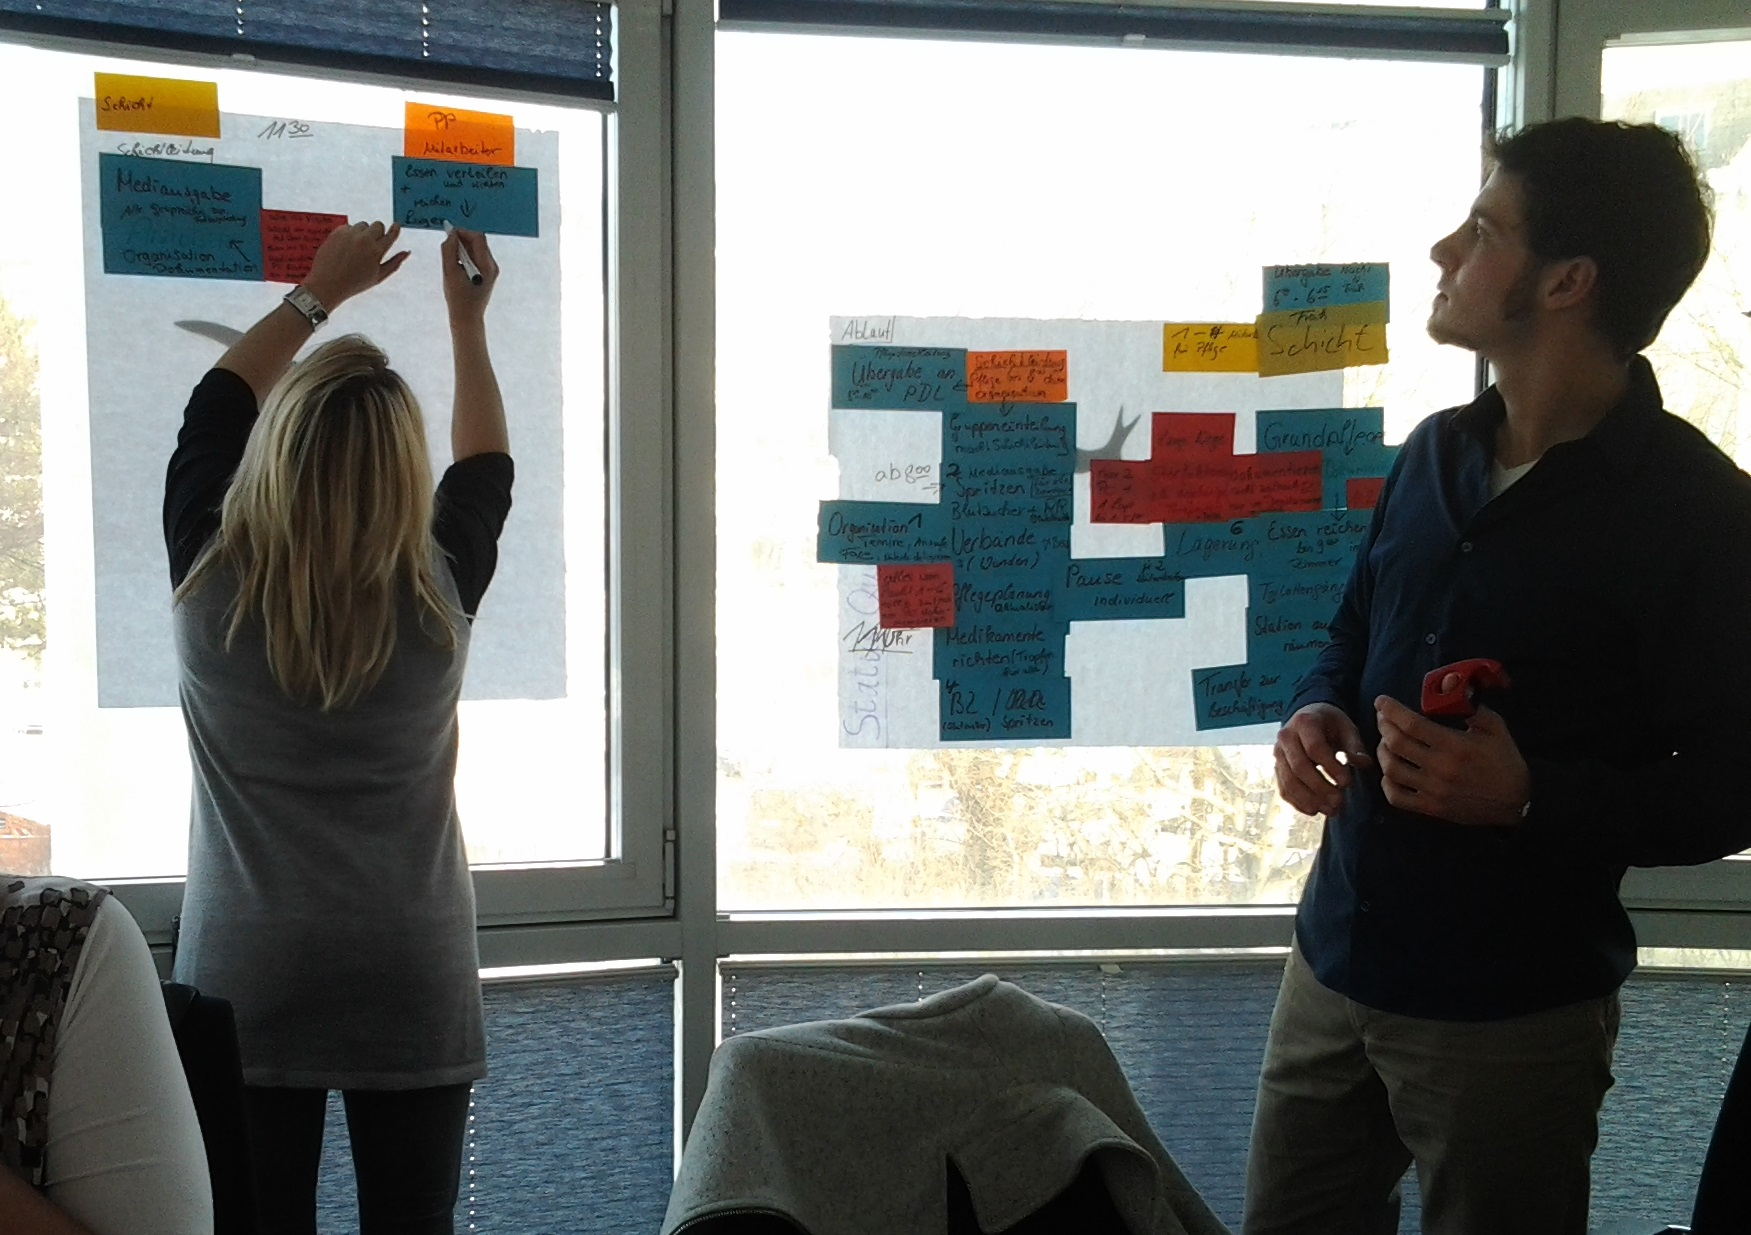
\includegraphics[width=8.5cm]{figures/eindruckSchulung.png} 
   \caption{Entwicklung eines Diagramms zur Ermittlung des Tagesablaufs mit den Teilnehmern}
   \label{fig:eindruckSchulung}
\end{wrapfigure}

Durch eine Analyse des momentanen Ablaufes in Zusammenarbeit mit den ausf�hrenden Kr�ften sollten St�rken und Schw�chen
mit besonderem Augenmerk auf der Dokumentation identifiziert werden. Zun�chst wurde hierzu der Tagesablauf der
Pflegekr�fte rekonstruiert und in einem Diagramm f�r bessere �bersichtlichkeit festgehalten. Ein Eindruck der Ermittlung
des Status Quo kann in Abbildung \ref{fig:eindruckSchulung} gewonnen werden. Das erstellte Diagramm zeigt prinzipiell
eine Sequenz von T�tigkeiten (blau), denen Probleme auf roten Karten zugeordnet wurden. Der genaue Ablauf des Tages ist
nicht entscheidend und wird hier nicht reproduziert, sondern lediglich die dadurch gewonnen Erkenntnisse
zusammengefasst. Ziel des Diagramms war es herauszufinden, an welchen Stellen in welchem Umfang dokumentiert werden
muss, welche Fehlerquellen sich im momentanen Ablauf ergeben und welche Aspekte verbessert werden k�nnten, um den Ablauf
im Bezug auf die Dokumentation zu vereinfachen.\\
Schnell kristallisierte sich heraus, dass der wichtigste und kritischste Faktor w�hrend der Arbeit der Pflegekr�fte
\textit{Zeit} ist. In der Konsequenz bedeutet dies, dass jede Ma�nahme, die mehr Zeit verschafft, positiv zu bewerten
ist und jede Verz�gerung des Ablaufs zu vermeiden ist.\\
Eine wichtige Erkenntnis ist, dass es nicht eine Reihe von T�tigkeiten gibt, die w�hrend \textit{eines} Besuchs beim
Patienten abgearbeitet werden, sondern dass w�hrend einer Schicht, zumindest im station�ren Bereich, mehrere Besuche beim
Patienten mit verschiedenen Aufgaben durchgef�hrt werden. Alle T�tigkeiten werden dem Personal in einer so genannten
\textit{Tagesstruktur} mitgeteilt, die im Laufe der Schicht abgearbeitet werden m�ssen. Es lassen sich bestimmte
T�tigkeitsbl�cke identifizieren, die in einer bestimmten zeitlichen Reihenfolge liegen wie z.B. die Grundpflege vor dem
Essen reichen, anschlie�end Transfer der Bewohner zu individuellen Besch�ftigungsprogrammen. Daneben gibt es eine Reihe
von T�tigkeiten, die nicht zu einem bestimmten Zeitpunkt erledigt werden m�ssen, sondern jeweils dann, wenn Bedarf
besteht. Hierzu geh�ren beispielsweise die Lagerung der immobilen Bewohner sowie Toiletteng�nge. Dokumentiert werden
muss alles, das entweder f�r die  sp�tere Abrechnung mit der Krankenkasse ben�tigt wird oder medizinisch relevant ist.
Medizinische Relevanz haben z.B. Toiletteng�nge, da der Stuhlgang st�ndig kontrolliert werden muss. Konnte bei einem
Patienten f�r eine gewisse Zeit kein Stuhlgang festgestellt werden, wird hieraus abgeleitet, dass dieser an einer
Verstopfung leidet und es werden abf�hrende Medikamente verabreicht.\\
In einer Schicht sind f�r ca. 40 Bewohner drei bis vier Pflegekr�fte sowie eine Schichtleitung zust�ndig. Die
Pflegekr�fte sind in der Regel nur f�r Pfleget�tigkeiten zust�ndig, w�hrend die Schichtleitung, meist eine examinierte
Krankenschwester, neben der Pflege der Bewohner au�erdem eine Reihe organisatorischer T�tigkeiten sowie Arzt-
und Angeh�rigenkommunikation erledigt. Um dieses Ma� an Arbeit zu schaffen, ist jedoch die Anzahl zu pflegender
Bewohner auf vier begrenzt, wobei die reinen Pflegekr�fte etwa acht Bewohner versorgen.

Nach Aussagen der Teilnehmer ist es wahrscheinlich, dass ausgebildete \acs{mfp}s nur noch �rztlich
�bertragene T�tigkeiten durchf�hren und keine Pflege mehr �bernehmen. Dies bedeutet, dass die Durchf�hrung und Dokumentation der
�bertragenen T�tigkeiten nicht zwischen den Pfleget�tigkeiten erfolgt, sondern in einem gesonderten Tagesablauf. Nimmt
man an, dass dieser Tagesablauf an den einer Schichtleitung angelehnt ist, wird auch hier jeder Klient mehrfach besucht,
da beispielsweise die Gabe von Medikamenten mehrfach pro Schicht erfolgt.

Die Dokumentation der T�tigkeiten wird direkt elektronisch durchgef�hrt, d.h. ohne die Ergebnisse auf Papier oder einem
anderen Medium �bergangsweise festzuhalten. Dokumentiert werden muss mit der daf�r vorgesehenen Software, die �ber drei
Computer verwendbar ist. Nur einer davon ist ein Laptop, die Dokumentation muss also in der Regel im Dienstzimmer an
den Desktop-PCs erfolgen. Da es nur drei PCs sind, die von vier bis f�nf Mitarbeitern inklusive Schichtleitung f�r die
Dokumentation aller Belange von 40 Patienten genutzt werden m�ssen, kommt es hier zwangsl�ufig zu Engp�ssen. Wenn dann
auch noch ein oder mehrere PCs defekt sind, versch�rft sich die Situation. Die Folge sind unproduktive
Wartezeiten, um die notwendige Dokumentation durchf�hren zu k�nnen, die von der Zeit, die f�r die Durchf�hrung der T�tigkeiten
gedacht war, abgeht.\\
Jede Pflegekraft versorgt in der Regel Patienten, die in nah beieinander liegenden R�umen untergebracht sind. So sollen
die Wege zwischen den Zimmern kurz gehalten werden und somit Zeit eingespart werden. Da alle Pflegekr�fte von den ihnen
zugewiesenen Zimmern h�ufig zur Dokumentation ins Dienstzimmer m�ssen, w�re es w�nschenswert, dass auch hier die
Wege kurz gehalten werden. Bei 40 Bewohnern auf einer Etage ist es jedoch nicht m�glich, allen Mitarbeitern Zimmer
direkt neben oder zumindest in unmittelbarer N�he des Computers zur Dokumentation zuzuweisen. Einige Mitarbeiter m�ssen
also jedes Mal relativ lange Wege auf sich nehmen. Eigentlich sind die Pflegekr�fte angehalten, jede T�tigkeit
unverz�glich zu dokumentieren, aber aufgrund der zur�ckzulegenden Wege werden meist mehrere T�tigkeiten durchgef�hrt,
bevor die Dokumentation erfolgt, um die Wegezeit zu sparen. Zwischen Durchf�hrung und dem Einpflegen des gemachten in
das Computersystem werden alle T�tigkeiten also zun�chst im Kopf "dokumentiert". Besonders morgens, bei der Durchf�hrung
der Grundpflege, die f�r acht Bewohner in etwa zwei Stunden Zeit in Anspruch nehmen darf, haben die Mitarbeiter keine
Kapazit�ten mehr frei, um die Dokumentation nach jedem Bewohner durchzuf�hren. Es kommen so enorm viele Informationen
�ber T�tigkeiten zusammen, die sich eine Pflegekraft merken muss. Hier kann es leicht passieren, dass T�tigkeiten, die
nicht routinem��ig durchgef�hrt werden oder sonstige Besonderheiten vergessen oder falsch dokumentiert werden. Dies kann
einerseits wirtschaftliche Konsequenzen haben, wenn Fehler bei abzurechnenden T�tigkeiten gemacht werden, andererseits
aber auch zu gesundheitlichen Sch�den f�hren, wenn hier relevante Informationen vergessen werden.\\
Neben dem reinen Zeitverlust durch die Wege zum Computer und zur�ck treten h�ufig "St�rfaktoren" auf dem Weg aus, die zu
weiterem Zeitverlust f�hren. Denn sobald eine Pflegekraft ein Zimmer verl�sst, kommt es h�ufig vor, dass sie von anderen
Bewohnern um etwas gebeten wird oder von Angeh�rigen in ein Gespr�ch verwickelt wird. Zwar sind dies Dinge, die neben
der reinen Dienstleistung ein wichtiger Bestandteil des Alten- und Pflegeberufs ist, da dies die menschliche Ebene
adressiert, jedoch bedeuten derartige Gespr�che und Zusatzleistungen rein rational gesehen einen kritischen Zeitverlust.
M�ssten weniger Wege ins Dienstzimmer angetreten werden, k�nnte das Potential f�r Ablenkungen in Zusammenhang mit
der Dokumentation gesenkt werden und somit effektiv Zeit eingespart werden.\\
Neben den genannten Problemen ist die Dokumentation an sich nach Aussage der Schulungsteilnehmer relativ aufwendig, da
h�ufig nicht nur eine T�tigkeit best�tigt werden muss, sondern zus�tzlich Daten eingepflegt werden m�ssen. Eine
effizientere Gestaltung w�re auch hier zur Einsparung der Dokumentationszeit w�nschenswert.\\
Im Zusammenhang mit Arztvisiten wurde als Problem genannt, dass ein Arzt die Pflegekraft h�ufig nach der aktuellen
Medikation oder sonstigen den Bewohner betreffenden Informationen fragt. Da bei acht zu betreuenden Bewohnern nicht alle
Informationen im Kopf behalten werden k�nnen und gerade bei Medikamenten exakte Informationen verf�gbar sein sollten,
muss auch hier ein Zusatzweg in das Dienstzimmer in Kauf genommen werden, um die Informationen am zentralen Computer
abzurufen.\\

Werden bei einer Arztvisite neue Medikamente verschrieben, Dosierungen ge�ndert oder bestehende abgesetzt, wird dies
h�ufig zun�chst handschriftlich direkt beim Bewohner dokumentiert. Handschriftliche Dokumentation bei derartig wichtigen
Werten wie Menge oder Name eines Medikaments kann schlimme Folgen haben, wenn die Anweisungen nicht gelesen werden
k�nnen oder missverstanden werden. Wegen Zeitdrucks entstehen so vermeidbare Fehler. Eine andere M�glichkeit der
Dokumentation, bei der Kommunikationsfehler durch unleserliche Schrift vermieden werden kann, ist hier sinnvoll.\\
Zur Aufgabe der Pflegekr�fte und auch der \acs{mfp}s geh�rt die Wunddokumentation. Momentan l�uft es so ab, dass mit
einer separat mitgef�hrten Kamera die Wunden fotografiert werden und die Bilder sp�ter am Computer der Akte des
Patienten hinzugef�gt werden. Zur Identifikation wird neben die Wunde ein Papierstreifen mit Name, Datum und der Gr��e
der Wunde gelegt. So kann zumindest, wenn das Bild angeschaut wird, kein Zuordnungsfehler passieren. Um die Bilddatei
der Patientenakte hinzuf�gen zu k�nnen, muss allerdings die Datei direkt ausgew�hlt werden. Hierzu muss sich der
Mitarbeiter die Nummer des entsprechenden Bildes merken und diese korrekt ausw�hlen. Klickt er beim Auswahlvorgang
daneben oder w�hlt aus einem anderen Grund das falsche Bild aus, kommt es zu einem Durcheinander bei den Wundfotos. Laut
Teilnehmern der Schulung kommt dies zwar selten vor, jedoch reicht die M�glichkeit der Verwechslung aus, um
Verbesserungspotential zu bieten.\\
Im Falle der Messung von Vitaldaten wie Blutdruck und Puls m�ssen genaue Werte festgehalten werden. Aus diesem Grund
werden die Werte vor Ort beim Bewohner auf Papier festgehalten und anschlie�end am Computer �bertragen. Auch hier kann
es ein Problem mit unsleserlichen Werten geben oder es werden schlichtweg Werte durch Vertippen oder zu gro�er Hektik
bei der �bertragung falsch in das System eingepflegt. Zur Verbesserung dieses Vorgangs m�sste das Zwischenmedium
abgeschafft werden oder sogar vollst�ndig von der manuellen Dokumentation abgesehen werden.

\begin{table}[htbp]
	\begin{tabularx}{\textwidth}{|X|c|}
		\hline
		\textbf{Identifiziertes Problem} & \textbf{Kritischer Faktor}\\
		\hline		
		H�ufiger Wechsel zwischen Patientenzimmer und Dienstzimmer zwecks Dokumentation & Zeit\\		
		\hline		
		Drei Computer zur Dokumentation bei 4 - 5 Mitarbeitern f�hren zu Engp�ssen und Wartezeiten & Zeit\\		
		\hline			
		Auf dem Weg von Dienstzimmer zum Patient und zur�ck treten h�ufig "St�rfaktoren" auf (Gespr�che mit Angeh�rigen,
		Fragen durch Patienten, Telefon) & Zeit\\		
		\hline		
		W�hrend der Arztvisite ist das Bereitstellen von Informationen zum Patienten wie die aktuelle Medikation meist mit
		einem Gang ins Dienstzimmer verbunden, da die Pflegekr�fte nicht alle Daten im Kopf haben k�nnen und die Daten auch
		nicht vor Ort im Zimmer abgerufen werden k�nnen. & Zeit\\		
		\hline		
		Die Dokumentation dauert wegen fehlender Autovervollst�ndigung oder vordefinierten Antworten relativ lange. & Zeit\\		
		\hline		
		Es werden nicht f�r jeden Bewohner direkt die durchgef�hrten T�tigkeiten dokumentiert, da dies zus�tzliche Wege zum
		Computer und eventuelle Wartezeiten bedeuten w�rde. Die Dokumentation erfolgt also nicht zeitnah und f�r mehrere
		Bewohner auf einmal. Da die Informationen auch nicht �bergangsweise auf Papier festgehalten werden (au�er die
		Viltaldaten-Messwerte), k�nnen hier bei der Dokumentation leicht Fehler durch vergessene oder falsche Informationen
		auftreten. & Qualit�t\\		
		\hline		
		Wundfotos k�nnten zur Patientenakte falsch zugeordnet werden, da sie mit einer externen Kamera aufgenommen wurden und
		erst sp�ter manuell der Akte hinzugef�gt werden. & Qualit�t\\		
		\hline		
		�bertragungsfehler bei auf Papier zwischennotierten Messwerten & Qualit�t\\		
		\hline		
		Anordnungen des Arztes wie beispielsweise eine ge�nderte Medikation werden oft vor Ort beim Patienten von Hand
		dokumentiert, um diese sp�ter in das Computersystem einzupflegen. Wegen Unleserlichkeit k�nnen hier Fehler mit
		gesundheitssch�dlichen oder sogar lebensbedrohlichen Folgen passieren. & Qualit�t\\		
		\hline
	\end{tabularx}
	\caption{Liste der identifizierten Probleme bei der Dokumentation von Pflegeleistungen in der Residenz Bad
	Friedrichshall}
	\label{tab:docuProbs}
\end{table}

Der bisher beschriebene Status Quo der Dokumentation von Pflegeleistungen und vereinzelt auch �rztlich �bertragbaren
T�tigkeiten hat einige Punkte mit Verbesserungspotential offenbart. Die Befragung hat die Annahme best�tigt, dass eine
Untersuchung sinnvoll ist, in wie fern eine st�rkere Unterst�tzung durch IT den Dokumentationsvorgang effizienter
und qualitativ hochwertiger machen kann. In Tabelle \ref{tab:docuProbs} werden die identifizierten Probleme noch einmal kurz
zusammengefasst und die damit verbundenen kritischen Faktoren benannt. 

\subsection{Anforderungen an CareNet\textit{mobile} aus Sicht der Zielnutzergruppe}
\label{subsec:anforderungen}

Im folgenden Abschnitt werden die in der Diskussion des Status Quo identifizierten Anforderungen an eine mobile L�sung
zur Unterst�tzung der Dokumentation aufgelistet und bewertet. Die Bewertung erfolgt danach, ob eine Anforderung bereits
vorher antizipiert wurde und falls ja, wie sie umgesetzt wurde. Falls es sich um eine neue Anforderung handelt, wird
�berpr�ft, ob sie �berhaupt umsetzbar ist und ob die Umsetzung f�r den Erfolg der Arbeit notwendig ist. Bei der Erhebung
der Anforderungen muss darauf hingewiesen werden, dass den Teilnehmern vorher die Rahmenbedingungen wie die Nutzung
eines Tablet-PCs und die damit verbundenen M�glichkeiten genannt wurden. Aus diesem Grund wurden manche Anforderungen
genannt, die nicht zwingend aus dem momentanen Tagesablauf hervorgehen, sondern mehr genannt wurden, weil es m�glich
gemacht werden kann. Es bestimmte also teilweise das Angebot die Nachfrage und nicht umgekehrt.

\begin{enumerate}
  \item \textit{Die Anwendung muss �bersichtlich strukturiert und intuitiv bedienbar sein.}
  		\par
  		\begingroup
  		\leftskip=1cm
  		\noindent Neben den fachlichen Anforderungen an die Anwendung wurde vor allem auf eine intuitive Bedienung und
  		�bersichtlichkeit geachtet, da dies als kritischer Faktor f�r die Akzeptanz der Anwendung angesehen wird. Mit der
  		in Abschnitt \ref{sec:basisanwendung} beschriebenen grafischen Oberfl�che soll den meist wenig technik-affinen
  		Nutzern das Erlernen der Bedienung erleichtert werden.
  		\par
  		\endgroup
  		
  	\item \textit{Die Tagesstruktur muss komplett pro Bewohner abrufbar sein.}
  		\par
  		\begingroup
  		\leftskip=1cm
  		\noindent Unter \textit{Tagesstruktur} verstanden die Teilnehmer der Schulung einen Plan, der alle zu versorgenden
  		Patienten und die auszuf�hrenden T�tigkeiten auflistet. Bisher wurde angenommen, dass die \acs{mfp}s eine Art
  		Tourenplan bekommen, nachdem sie arbeiten. Es wurde also bisher vor allem von einer zumindest teilweisen ambulanten
  		Erbringung von Dienstleistungen ausgegangen. Da die Konzepte einer Tagesstruktur und eines Tourenplans aber
  		prinzipiell gleich sind, muss nur entsprechend dem Kontext (station�re oder ambulante Dienste) die Namensgebung
  		angepasst werden, um den Nutzern m�glichst viele bekannte Elemente in der neuen Technologie zu bieten.
  		\par
  		\endgroup
  		
  	\item \textit{Die Dokumentation ausgef�hrter T�tigkeiten muss im Zimmer/vor Ort m�glich sein.}
  		\par
  		\begingroup
  		\leftskip=1cm
  		\noindent Diese Anforderung wurde implizit dadurch erf�llt, dass in der Aufgabenstellung die Nutzung von Tablet-PCs
  		gefordert war. Durch die mobile Verwendbarkeit ist eine Dokumentation im Zimmer m�glich.
  		\par
  		\endgroup
  		
  	\item \textit{Die Patientenakte sollte auf dem Endger�t vollst�ndig abrufbar sein.}
  		\par
  		\begingroup
  		\leftskip=1cm
  		\noindent Dass Informationen zum Patienten abrufbar sein m�ssen, wurde zu Beginn angenommen. Neben den
  		Grundinformationen zum Finden des Patienten wie Name und Adresse sind auch Informationen zu Angeh�rigen, zust�ndigen
  		�rzten und aktueller Medikation gew�nscht. Da CareNet diese Informationen bereits anbietet, wurde zumindest f�r die
  		Stammdaten (Name, Adresse, Kontaktm�glichkeit) eine Repr�sentation in den Plug-Ins "Kontakte" und Touren
  		vorbereitet. Eine vollst�ndige Implementierung aller m�glichen Daten erfolgt im Rahmen dieser Arbeit nicht, da eine
  		Vorbereitung zum Einf�gen weiterer Daten das Ziel grunds�tzlich erf�llt.
  		\par
  		\endgroup
  		
  	\item \textit{Die Patientenakte sollte vor Ort beim Patienten anpassbar sein.}
  		\par
  		\begingroup
  		\leftskip=1cm
  		\noindent Von den Teilnehmern wurde gew�nscht, dass die Daten des Patienten auf dem Tablet-PC editierbar sein
  		sollten. Da dies aber auch in CareNet m�glich ist und anzunehmen ist, dass nicht bei jedem Besuch beim Patienten die
  		Daten angepasst werden m�ssen, wurde entschieden, dass eine Implementierung dieser Anforderung zum jetzigen
  		Zeitpunkt keinen Mehrwert bringt und deswegen nicht umgesetzt wird. Sollte die Anwendung sp�ter tats�chlich zum
  		Einsatz kommen, ist die Umsetzung einer Editierfunktion aber sicherlich zu empfehlen, da sie den Nutzungskomfort
  		steigert.
  		\par
  		\endgroup
  		
  	\item \textit{Die Patientenakte sollte Bilder vom Patienten enthalten, um Verwechslungen bei gleichem Namen
  	 	          (z.B. bei einem Ehepaar) im gleichen Zimmer zu vermeiden.}
  		\par
  		\begingroup
  		\leftskip=1cm
  		\noindent Die Verwendung von Bildern in der Patientenakte und in der Tagesstruktur wurde zu Beginn der Arbeit
  		bereits diskutiert. Die Anforderung wurde allerdings verworfen, da Bilder der Patienten zus�tzliche
  		Anforderungen an den Datenschutz in CareNet gestellt h�tten, was in Anbetracht der Bearbeitungszeit der
  		Master-Arbeit nicht zu realisieren gewesen w�re.
  		\par
  		\endgroup
  	  		
  	\item \textit{M�glichkeit bei jeder T�tigkeit anzugeben, dass diese nicht ausgef�hrt wurde und warum.}
		\par 
		\begingroup 
		\leftskip=1cm 
		\noindent Die Teilnehmer der Schulung gaben an, dass es immer wieder sein kann, dass aus irgend einem Grund eine
		gefroderte Leistung nicht erbracht werden kann. Damit die Aufgaben des Tages trotzdem als erf�llt angesehen werden
		k�nnen, muss eine T�tigkeit mi Begr�ndung als "nicht erbracht" markiert werden k�nnen.  
		\par 
		\endgroup
		
	\item \textit{Zeitlich nicht planbare und pl�tzlich zu erbringende T�tigkeiten wie die Hilfe beim Toilettengang
  				  m�ssen der Tagesstruktur am Tablet-PC hinzuf�gbar sein.}
  		\par
  		\begingroup
  		\leftskip=1cm
  		\noindent Die Erg�nzung von Dienstleistungen, die von der geplanten Tagesstruktur abweichen, wurde bereits im ersten
  		Anforderungskatalog aufgenommen, da angenommen wurde, dass die Arbeit mit Menschen immer unvorhergesehene
  		T�tigkeiten n�tig machen kann. Aus Zeitgr�nden konnte diese wichtige Funktionalit�t allerdings nicht mehr im Rahmen
  		dieser Arbeit implementiert werden.
  		\par
  		\endgroup	
  	
  	\item \textit{Vitaldaten (Blutdruck, Puls, Schmerzmanagement, Gewicht) m�ssen am Tablet-PC erfassbar sein.}
  		\par
  		\begingroup
  		\leftskip=1cm
  		\noindent Die Anforderung der Erfassung von Vitaldaten musste bereits im VitaBit Projekt umgesetzt werden und wurde
  		aus diesem Grund auch in den Anforderungskatalog von \app aufgenommen. Allerdings beschr�nken sich die erfassbaren
  		Daten bisher auf Blutdruck und Puls. Eine Erfassung von Gewicht und ein Schmerzmanagement ist jedoch m�glich, wird
  		aber im Rahmen dieser Arbeit nicht mehr implementiert.
  		\par
  		\endgroup
  	
  	\item \textit{Statistiken �ber alle Vitaldaten w�ren hilfreich (Bsp: Verlauf des Gewichts seit Einlieferung).}
  		\par
  		\begingroup
  		\leftskip=1cm
  		\noindent Eine genaue Zustands�nderung bei einer Person l�sst sich meist nur mit Hilfe von Vergleichswerten
  		vergangener Erhebungen identifizieren. Aus dieser Annahme wurde bei der initialen Anforderungsevaluation abgeleitet,
  		dass es hilfreich sein k�nnte, vorangegangene Messungen von Vitalparametern in einer �bersichtlichen Statistik
  		abfragen zu k�nnen. Die Implementierung einer solchen Funktionalit�t war zun�chst geplant, musste jedoch wegen der
  		K�rze der Zeit aus der Agenda genommen werden. F�r einen produktiven Einsatz von \app wird diese Funktionalit�t
  		allerdings als notwendig angesehen, um einen klaren Vorteil gegen�ber manueller Dokumentation und Auswertung der
  		erhobenen Daten zu bieten.
  		\par
  		\endgroup
  		
  	\item \textit{Automatische Plausibilit�tspr�fung von eingegebenen Messwerten (Z.B. Puls > 250 $\Rightarrow$
  	Warnung).}
  		\par
  		\begingroup
  		\leftskip=1cm
  		\noindent Automatische Plausibilit�tspr�fungen sind eine zentrale M�glichkeit zur Steigerung der Qualit�t bei
  		EDV-gest�tzter Dokumentation. Diese Art der �berpr�fung wurde von Anfang an als w�nschenswert angesehen, jedoch ist
  		dies ein Merkmal, das erst implementiert werden kann, wenn grunds�tzlich die Dokumentation funktioniert. Da
  		die Umsetzung der gesamten Architektur und der Basisfunktionalit�ten schon die gesamte Bearbeitungszeit in Anspruch
  		genommen hat, wurde eine Plausibilit�tspr�fung nur in den Anforderungen f�r den Fall einer Weiterf�hrung des
  		Projektes aufgenommen. Je nach Komplexit�t der Werte ist die Implementierung zwar sehr aufwendig, aber m�glich.
  		\par
  		\endgroup
  		
	 \item \textit{Warnungen, wenn gemessene Werte kritisch sind oder wenn dokumentierte T�tigkeiten auf m�gliche
	 Gefahren f�r den Bewohner/Patienten hindeuten (beispielsweise, wenn f�r einen Patienten schon l�nger kein Stuhlgang
	 mehr dokumentiert wurde).}
		\par 
		\begingroup 
		\leftskip=1cm 
		\noindent Diese Anforderung ist �hnlich zu bewerten wie die Plausibilit�tspr�fung, da sie prinzipiell die gleichen
		Voraussetzungen haben. Auch hier wird eine Logik �ber die grundlegende Dokumentation hinaus ben�tigt, welche erst zu
		einem sehr "reifen" Zeitpunkt der Entwicklung implementiert werden kann. Dieser konnte w�hrend dieser Arbeit noch
		nicht erreicht werden. Logik, die aus den dokumentierten Daten Schl�sse zieht, sollte unbedingtes Ziel der Entwicklung
		sein.
		\par 
		\endgroup
		
	\item \textit{Wundfotos sollten mit der internen Kamera des Tablet-PCs aufnehmbar sein und direkt dem Patienten
  		zugeordnet werden.}
  		\par
  		\begingroup
  		\leftskip=1cm
  		\noindent Diese Anforderung wurde nicht aktiv von den Schulungsteilnehmern ge�u�ert, sondern als m�gliche
  		Funktionalit�t aufgrund der Eigenschaften eines Tablet-PCs vorgeschlagen. Der Vorschlag wurde positiv
  		aufgenommen und als m�glicherweise komfortabel und n�tzlich bewertet. Einerseits aus dem Grund, weil keine
  		zus�tzlich Kamera mehr mitgef�hrt werden muss, und andererseits weil der Arbeitsschritt der manuellen Zuordnung
  		wegf�llt und somit Zeit gespart wird. Daneben f�llt auch die Fehlerquelle der manuellen Zuordnung der Bilder zur
  		Patientenakte weg. Diese Funktion wurde in der aktuellen Version der Anwendung implementiert.
  		\par
  		\endgroup
  	
  	\item \textit{Die Pflegestandards des Hauses sollten auf dem Tablet-PC abrufbar sein.}
  		\par
  		\begingroup
  		\leftskip=1cm
  		\noindent Diese Anforderung hat rein informativen Charakter und soll als Hilfestellung dienen, wenn unklar ist, wie
  		in einem bestimmten Fall vorgegangen werden soll. Da sich die Teilnehmer �ber die Notwendigkeit dieser Funktion
  		nicht einig waren, da die meisten Pflegekr�fte bereits �ber langj�hrige Erfahrung verf�gen und die Vorg�nge ohnehin
  		kennen, wurde die Anforderung nicht aufgenommen. Au�erdem liefert sie keinen Mehrwert zur Dokumentation, welche das
  		Kernthema der Evaluation ist.
  		\par
  		\endgroup
  		
  	\item \textit{Spracherkennung zur Eingabe von Freitext.}
  		\par
  		\begingroup
  		\leftskip=1cm
  		\noindent Eine Spracherkennung zur Eingabe von Freitext wurde h�ufig gew�nscht, da die Eingabe von Freitext �ber die
  		virtuelle Tastatur als zu langwierig angesehen wurde. Zwar bieten die neueren Betriebssysteme von Android und iOS
  		die M�glichkeit der Spracheingabe, jedoch ist hierzu eine Internetverbindung notwendig, was nicht immer
  		gew�hrleisten werden kann. Der initiale Anforderungskatalog enthielt die Anforderung, dass \app auch ohne
  		Internetverbindung funktionieren muss, was mit einer internetabh�ngigen Spracherkennung nicht zu vereinbaren ist.
  		Eventuell w�re es eine M�glichkeit, eine eigene Spracherkennung zu implementieren oder eine vorhandene zu
  		lizensieren und auf dem Endger�t verf�gbar zu machen, jedoch ist zu vermuten, dass der zeitliche und finanzielle Aufwand hierf�r
  		so hoch w�re, dass sich die Umsetzung kaum lohnt. Denkbarer w�re eine Einschr�nkung der Spracherkennung auf den
  		station�ren Dienst, wenn in einer Einrichtung ein Drahtlosnetzwerk verf�gbar ist.
  		\par
  		\endgroup
  		
  	 \item \textit{Abrufen des Tropfenplans auf dem Tablet-PC.}
  		\par
  		\begingroup
  		\leftskip=1cm
  		\noindent Der Tropfenplan ist eine Auflistung aller ben�tigten fl�ssigen Medikamente einer Schicht. Er wird dazu
  		verwendet, die Medikamente in einem Arbeitsschritt an der Medikamentenausgabe zusammenzustellen. Prinzipiell k�nnte
  		diese Anforderung mit vertretbarem Aufwand implementiert werden, jedoch fehlt hierf�r die Voraussetzung in CareNet,
  		da die fl�ssigen Medikamente nicht gesondert in der Patientenakte verf�gbar sind. Weil der Tropfenplan keine
  		Relevanz f�r die Dokumentation hat, sondern nur f�r die Vorbereitung der T�tigkeiten ben�tigt wird, wird die
  		Anforderung zwar in die m�glicherweise sp�ter umzusetzenden Liste von Anforderungen aufgenommen, in dieser Arbeit
  		aber nicht weiter beachtet.
  		\par
  		\endgroup
  	
	\item \textit{Notrufknopf zum Absetzen eines Telefonanrufs f�r die ambulante Dienste.}
  		\par
  		\begingroup
  		\leftskip=1cm
  		\noindent In einem vorangegangenen Projekt wurde ein Notrufknopf zum schnellen Absetzen von Notrufen eingebaut. Auf
  		die Frage, ob dies auch eine w�nschenswerte Funktionalit�t f�r \app sei, sagten die Teilnehmer, dass dies eigentlich
  		nur im ambulanten Bereich sinnvoll w�re, da in der Residenz ohnehin Telefone schnell verf�gbar w�ren. Da der Fokus
  		momentan auf einem Einsatz im station�ren Bereich liegt, wird kein Notrufknopf implementiert. Au�erdem setzt das
  		voraus, dass der Tablet-PC Telefonanrufe absetzen kann. Das verteuert die Hardware und macht weitere wirtschaftliche
  		Untersuchungen erforderlich.
  		\par
  		\endgroup
  		
  	\item \textit{"Rote Liste" auf Tablet-PC abrufbar.}
  		\par
  		\begingroup
  		\leftskip=1cm
  		\noindent Die "Rote Liste" stellt eine Sammlung aller zugelassenen Medikamente dar, in der Wirkung und
  		Wechselwirkungen mit anderen Medikamenten beschrieben werden. Einige Teilnehmer w�nschten sich, dass diese Liste auf
  		dem Tablet-PC abrufbar sei. Da es sich hierbei aber eigentlich um ein Buch eines Anbieters handelt, d�rfen die
  		Inhalte des Buchs nicht ohne Lizenzzahlungen in der Anwendung verwendet werden. Zudem ist unklar, ob die Verwendung
  		�berhaupt erlaubt w�rde, da die Implementierung einer App zum Zugriff auf die Inhalte eigentlich Aufgabe des
  		Verlages w�re. Da diese Funktionalit�t auch keine Relevanz f�r die Dokumentation hat, wird sie nicht in den
  		Anforderungskatalog aufgenommen.
  		\par
  		\endgroup
  		
  	\item \textit{Tablet-PCs mit Glasoberfl�che, um diese leicht reinigen zu k�nnen.}
  		\par
  		\begingroup
  		\leftskip=1cm
  		\noindent Hygiene ist im medizinischen und pflegerischen Bereich ein wichtiger Aspekt. Da die Tablet-PCs mit in die
  		Zimmer oder Wohnungen der Bewohner/Klienten genommen werden, m�ssen diese nach jedem Besuch desinfiziert werden. Die
  		Oberfl�che sollte deswegen aus Glas sein, da die Desinfektionsmittel eine Kunststoffoberfl�che bei h�ufigem Kontakt
  		m�glicherweise sch�digen. Die Anforderung war zu Beginn der Arbeit zwar nicht bekannt, wurde aber erf�llt, da die
  		Implementierung testweise auf Samsung Galaxy Tabs I und II erfolgte, welche eine Glasoberfl�che besitzen. Die
  		Anforderung wurde in den Gesamtkatalog aufgenommen.
  		\par
  		\endgroup 	
\end{enumerate}

\subsection{Ergebnisse des Abschlussfragebogens}

Nachdem die Anforderungen an \app mit den Teilnehmern evaluiert wurden, wurde der Stand der Entwicklung der Anwendung
vorgestellt. Fertiggestellt war zu diesem Zeitpunkt die Einstiegsseite mit der �bersicht �ber die verf�gbaren Plug-Ins,
das Plug-In \textit{Kontakte} und im Plug-In \textit{Touren} konnte bereits eine einfache Tagestruktur abgerufen
werden, sprich pro Bewohner T�tigkeiten, die nur Best�tigt werden m�ssen. Zudem konnte jede T�tigkeit mit
Begr�ndung als "nicht durchgef�hrt" markiert werden. Die Dokumentation von Wunden per Foto und die Erfassung von
Vitaldaten war noch nicht m�glich. Es konnte jedoch zu jedem Patienten eine erste Version der Patientenakte abgerufen
werden.\\
Nach der Vorf�hrung, bei der jedes Team auf dem eigenen Tablet-PC die Anwendung ausprobieren konnte, wurde ein
Fragebogen verteilt, mit dem die Benutzbarkeit, der Lernaufwand zur Nutzung der Anwendung und der erwartete Nutzen
durch den Einsatz bei der t�glichen Arbeit abgefragt wurde. Der verwendete Fragebogen ist im Anhang
\ref{app:abschlussfragebogen} zu finden. Als Basis f�r die verwendeten Fragen wurde auf den bereits validierten
Fragebogen des \acs{utaut}-Modells \cite{utaut} zur�ckgegriffen. \acs{utaut} steht f�r \textit{\acl{utaut}} und stellt ein
Rahmenwerk zur Bewertung des Nutzens und der Akzeptanz durch den Endnutzer dar. Da die Fragen im Original auf englisch
sind, mussten diese zun�chst ins Deutsche �berf�hrt werden. \cite[S. 50 ff.]{masterMathias} hat dies zur Evaluation der
Software CareCM der nubedian GmbH, auf der CareNet aufbaut, bereits getan. Die hier verwendeten Fragen sind an diese
�bersetzung angelehnt und wurden an die Belange der Bewertung von \app angepasst. Wie der Fragebogen zur Ermittlung der
Vorkenntnisse wurde auch der Abschlussfragebogen schriftlich und anonym von jedem Teilnehmer ausgef�llt.

\begin{figure}[h]
	\centering
	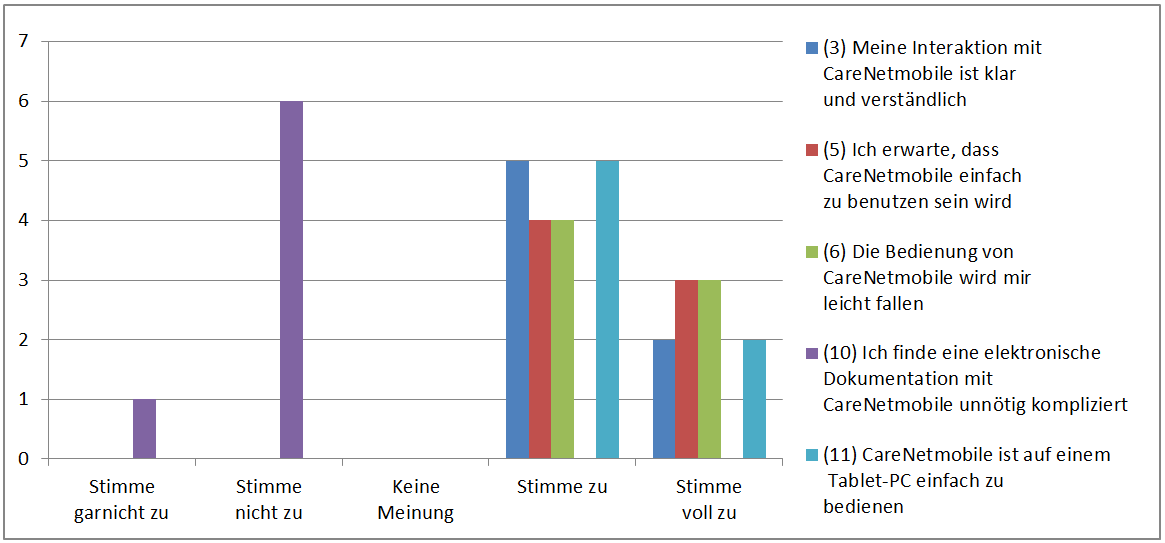
\includegraphics[width=\textwidth]{figures/StatBenutzbarkeit.png}
	\caption{Ergebnisse der Fragen zur Benutzbarkeit von \app.}
	\label{fig:statBenutzbarkeit}
\end{figure}

Die Ergebnisse der Fragen zur Benutzbarkeit von \app sind in Abbildung \ref{fig:statBenutzbarkeit} aufgef�hrt.
Den Fragen, ob die Anwendung leicht zu bedienen sein wird (5, 6 und 11), ist von allen Teilnehmern zugestimmt worden.
Der Inhalt der drei Fragen �berschneidet sich aus dem Grund, um festzustellen, ob die Teilnehmer nur zuf�llig angekreuzt
haben.Da alle Fragen von allen Teilnehmern mit gleicher positiver Tendenz angekrauzt wurden, ist anzunehmen, dass die
Fragen verstanden und konsistent beantwortet wurden. Auch der Frage, ob die Interaktion mit \app (3) verst�ndlich ist,
wurde zugestimmt. Dass "nur" f�nf von sieben Teilnehmern zugestimmt und nicht voll zugestimmt, l�sst darauf schlie�en,
dass gewisse Anpassungen der grafischen Oberfl�che notwendig sind, um eine volle Zufriedenheit zu erreichen. Die
Gegenfrage, ob eine elektronische Dokumentation mit \app unn�tig kompliziert sei, wurde konsequenter Weise im Vergleich
zu den anderen Antworten verneint. Bei dieser Frage stimmte nur eine Teilnehmerin voll zu, was vermutlich auf den im
ersten Fragebogen (vgl. Abbildung \ref{fig:casResults}) festgestellten Respekt gegen�ber einer neuen Technologie
zur�ckzuf�hren ist.

\begin{figure}[ht]
	\centering
	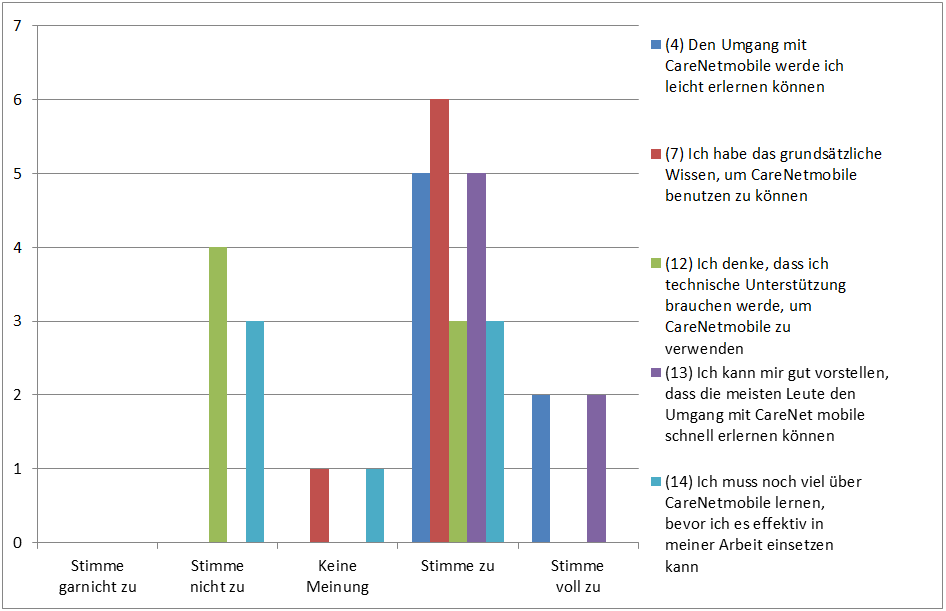
\includegraphics[width=\textwidth]{figures/StatLernaufwand.png}
	\caption{Ergebnisse der Fragen zum ben�tigten Vorwissen und Lernaufwand zur Nutzung von \app.}
	\label{fig:statLernaufwand}
\end{figure}

Abbildung \ref{fig:statLernaufwand} zeigt das Ergebnis der Fragen zum erwarteten Lernaufwand zur Nutzung von \app. Die
Fragen, ob die Teilnehmer selbst den Umgang mit der Anwendung leicht lernen k�nnen (4) und wie sie dies bei anderen
einsch�tzen (13), wurde positiv beantwortet. Die Angabe, das sechs von sieben Teilnehmern meinen, das grunds�tzliche
Wissen zu haben, um \app zu benutzen (7), spricht daf�r, dass die Bedienung der Anwendung als �hnlich intuitiv angesehen
wird wie die Bedienung sonstiger Anwendungen des Tablets, da bisher keine spezielle \app Schulung erfolgt ist. Bei der
Frage nach zus�tzlicher technischer Unterst�tzung (12) waren sich die Teilnehmer nicht einig. �hnlich unentschieden
fielen die Antworten bei der These aus, dass die Teilnehmer vor einem effektiven Einsatz noch viel zus�tzlich lernen
m�ssten (14). Es ist zu vermuten, dass eine Aussage, dass keine technische Unterst�tzung mehr n�tig w�re, eher ein
Ausdruck von technischem Selbstvertrauen ist als das tats�chlich vorhandene Wissen \app zu verwenden. Erwartet worden
war hier, dass eine deutliche Mehrheit der Teilnehmer ausstehenden Schulungsbedarf sieht und Unterst�tzung f�r Notwendig
h�lt. Dies wurde erwartet, da erstens keine echte Schulung statt gefunden hat und au�erdem nur ein Teil der geforderten
Funktionalit�t implementiert war.

\begin{figure}[hb]
	\centering
	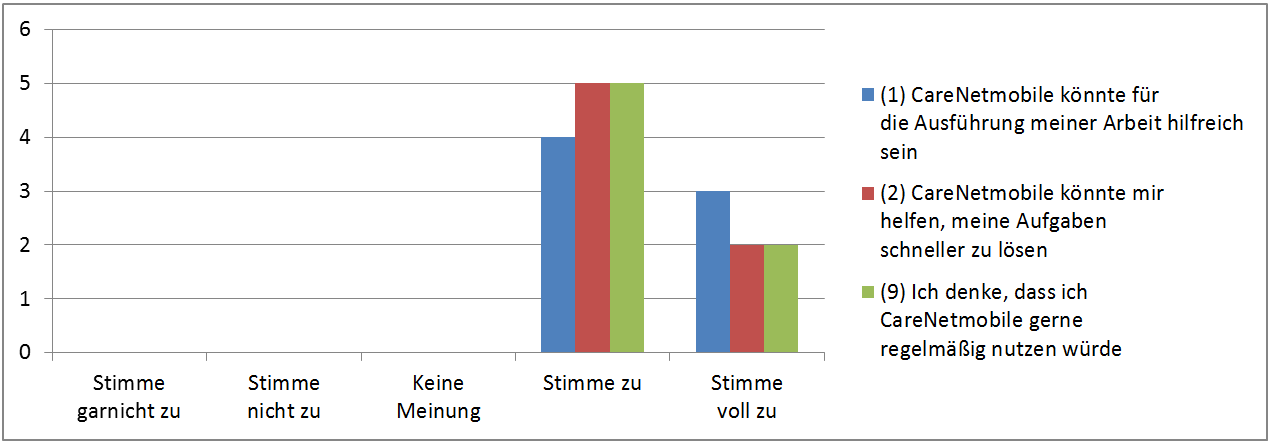
\includegraphics[width=\textwidth]{figures/StatAkzeptanz.png}
	\caption{Ergebnisse der Fragen zu potentiellem Nutzen und Akzeptanz von \app.}
	\label{fig:statAkzeptanz}
\end{figure}

Die Fragen zu Nutzen und Akzeptanz von \app sind sehr positiv ausgefallen. Alle Teilnehmerinnen sagten aus, dass die
Anwendung grunds�tzlich hilfreich sein k�nnte (1) und dass durch sie die Arbeit effizienter erledigt werden und somit
Zeit eingespart werden k�nnte (2). Die Teilnehmerinnen sagten sogar durchweg aus, dass sie die Anwendung gerne
regelm��ig nutzen w�rden, was ein sehr gutes Ergebnis des Schulungstages ist, da diese Aussage daf�r spricht, dass
eventuell vorhandene Widerst�nde und Vorbehalte, die zu Beginn identifiziert wurden (vgl. \ref{subsec:vorwissen}, erfolgreich
�berwunden wurden. Obwohl zun�chst gewisse �ngste aufgrund der geringen Technikaffinit�t gegen�ber der neuen Technologie
bestanden, lehnte keine Teilnehmerin die Nutzung grunds�tzlich ab.

Lediglich die Frage nach der Freiwilligkeit der Verwendung von \app wurde aus der Bewertung des Fragebogens
herausgenommen. Eigentlich war diese Frage daf�r gedacht herauszufinden, ob die Alten- und Krankenpfleger durch
R�ckmeldung einen Einfluss auf die Art der Dokumentation haben, jedoch zeigen die widerspr�chlichen Antworten, dass
keine Einigkeit herrscht, obwohl die meisten Teilnehmer in der gleichen Einrichtung mit den gleichen Vorgesetzten
arbeiten. Aus dem Ergebnis wurde geschlossen, dass die Frage missverst�ndlich gestellt war und gegen die g�ngige
Oganisationsstruktur in den Einrichtungen sprach, die meist hierarchisch gepr�gt ist. Aus diesem Grund wurde die Frage
nicht ber�cksichtigt.

Aufgrund der Ergebnisse des Abschlussfragebogens und des gewonnen Eindrucks kann die Schulung als grunds�tzlich
erfolgreich bewertet werden. Es konnte einerseits eine Reihe von Anforderungen gesammelt werden, andererseits konnte die
Akzeptanz der bisher entwickelten Idee an einer ersten Endnutzergruppe getestet werden.  Das Ziel, bei den Teilnehmern
eine gewisse Begeisterung f�r die Tablet-Technologie zu wecken und daraus mit einer positiven Stimmung in die
Anforderungsevaluation zu starten ist gelungen. Es war sehr erfreulich zu erfahren, dass die initialen Ideen und
Anforderungen nicht v�llig in die falsche Richtung gingen, sondern im Grunde den Nerv und die Notwendigkeiten der
Teilnehmer trafen. Die Evaluation der Anforderungen in Abschnitt \ref{subsec:anforderungen} hat gezeigt, dass nur wenige
in der Schulung genannte Anforderungen neu waren und dass an bestehenden Anforderungen nur geringe �nderungen
vorgenommen werden mussten. Da einige der neuen Anforderungen nichts mit dem eigentlichen Ziel der Dokumentation der
erbrachten Leistungen zu tun hat, wie z.B. die Verf�gbarkeit eines Tropfenplans oder eine Spracherkennung, wurden die
meisten neuen Anforderungen verworfen oder f�r eine eventuelle Weiterentwicklung zur�ckgestellt. Die �brigen
Anforderungen zusammen mit den technischen Voraussetzungen aus Kapitel \ref{ch:anforderungsanalyse} ergeben eine gute
Basis zur Entwicklung einer Anwendung, die Chancen hat, bei einer Weiterentwicklung zur Marktreife vom zust�ndigen Personal
akzeptiert zu werden und einen echten Mehrwert bei der Dokumentation �rztliche �bertragener T�tigkeiten zu liefern.


		   

\chapter{Fazit}
\label{ch:fazit}

Zu Beginn dieser Master-Arbeit war das Ziel die Erstellung einer lauff�higen mobilen Anwendung, die Angeh�rige der
alten- und Pflegeberufe darin unterst�tzen sollte, an sie delegierte �rztliche T�tigkeiten zu dokumentieren. Die Daten
sollten an das zentrale System \textit{CareNet} �bermittelt werden, sodass der Arzt, der die T�tigkeiten in Auftrag
gegeben hat, eine zeitnahe Kontrolle durchf�hren konnte.\\
Dieses Ziel konnte in der zur Verf�gung stehenden Bearbeitungszeit nicht in vollem Umfang erreicht werden, jedoch
konnten die wesentlichen Anforderungen umgesetzt werden. Eine Kernanforderung war, die Anwendung durch einen modularen
Aufbau flexibel und an ge�nderte Rahmenbedingungen anpassbar zu gestalten. Technologisch war die einzige Vorgabe, dass
moderne Tablet-PCs eingesetzt werden sollten. Dies erforderte einen zus�tzlichen Evaluationsprozess der am besten
geeigneten Technologie zur Erstellung einer mobilen Anwendung. Der Vergleich von nativ entwickelten Anwendungen, WebApps
und hybriden Anwendungen ergab, dass der hybride Ansatz trotz eventueller die Performanz betreffender Nachteile die
beste Basistechnologie sei. Das entscheidende Argument war die potenzielle Portierbarkeit der Anwendung auf verschiedene
Plattformen (Android, iOS, Windows Phone), da die endg�ltig zu verwendende Hardware noch nicht fest stand.\\
Zur Realisierung der Anpassbarkeit der Anwendung wurde eine Plug-In-Architektur gew�hlt, bei der jegliche f�r den
Endnutzer zu verwendende Funktionalit�t in Plug-Ins gekapselt werden sollte. Die Architektur konnte auf Basis von
JavaScript, HTML und CSS umgesetzt werden, jedoch nahm der Entwurf und die Implementierung mehr Zeit in Anspruch, als
zun�chst gesch�tzt wurde. Zwar konnten trotz dieser Verz�gerung die wesentlichen Funktionen umgesetzt werden, jedoch
mussten manche w�nschenswerte Eigenschaften aus Zeitgr�nden zur�ckgestellt werden. Implementiert werden konnte ein Plug-In zum
Abrufen von Kontaktdaten aus CareNet und ein Plug-In zur Darstellung einer Tour f�r eine \acl{mfp}, die die einzelnen
Stationen (Klienten) sowie die zu erbringenden Leistungen enthielt. Bei den Leistungen wurden auf Basis der
Anforderungsanalyse drei Leistungstypen identifiziert: Standardleistungen, die nur eine Best�tigung ben�tigen,
eine Wunddokumentation, mit der eine Bilddatei verkn�pft werden muss und eine Vitalwerterfassung, mit der Messwerte von
Blutdruck und Puls verbunden werden m�ssen. Standardleistungen und Wunddokumentation konnte den Anforderungen
entsprechend umgesetzt werden, jedoch sollte die Vitalwerterfassung durch den Anschluss von Messger�ten �ber Bluetooth
automatisiert werden, was nicht mehr realisiert werden konnte. Die Erfassung von Vitalwerten ist momentan nur �ber
manuelle Eingabe m�glich. Eine weitere geplante Funktionalit�t, die aus Zeitgr�nden nicht mehr implementiert werden
konnte, ist das Hinzuf�gen ungeplanter Leistungen wie Toiletteng�nge zu einer Station.\\
Die bisher entwickelte mobile Anwendung bildet die notwendige Grundfunktionalit�t ab (bis auf die vorher genannten
Punkte), um in CareNet zentral definierte Leistungen zu dokumentieren. W�hrend der Anforderungsanalyse konnten
allerdings noch einige Erweiterungsm�glichkeiten identifiziert werden, die \app attraktiver machen w�rden.
Hierzu z�hlen

\begin{itemize}
  \item Navigation zum Klienten per GPS, entweder in die Anwendung integriert oder Nutzung externer Navigationsprogramme
  \item Plausibilit�tspr�fung von eingegebenen Werten
  \item Warnungen bei eingegebenen kritischen Werten oder wenn Daten eines Klienten auf einen kritischen Zustand
  schlie�en lassen (beispielsweise wenn eine bestimmte Zeit kein Toilettengang dokumentiert wurde)
  \item Nutzung der per GPS ermittelten Position, um eine Behandlung auf dem Tablet-PC zu schlie�en, sobald sich die
  behandelnde \acs{mfp} vom Einsatzort entfernt
  \item Autovervollst�ndigung und Drop-Down-Listen zur Beschleunigung der Dokumentation von Standardf�llen
  \item Integration einer Telefonfunktion f�r Notrufe und R�ckfragen (Umsetzbarkeit hardwareabh�ngig)
\end{itemize}

Die Realisierung von \app auf Basis einer Plug-In-Architektur bietet eine Vielzahl von Erweiterungsm�glichkeiten. Neben
einer Erweiterung der Funktionen zur Dokumentation k�nnten auch v�llig andere Anwendungsfelder von CareNet oder
verwandten Produkten der nubedian GmbH mobil verf�gbar gemacht werden, da diese �ber die gleich \acs{rest}-Schnittstelle
kommunizieren. Durch die Kapselung von Funktionalit�t innerhalb eines Plug-Ins k�nnten beispielsweise Vorg�nge, Termine
oder sonstige Daten mit einer individuellen grafischen Oberfl�che dargestellt werden, ohne Implementierungen anderer
Plug-Ins zu beeinflussen. Da die Plug-Ins �ber eine Konfigurationsdatei der Basisanwendung hinzugef�gt werden, ist
au�erdem die M�glichkeit gegeben, einen Autorisierungsmechanismus zu implementieren, mit dem bestimmten Personen in
Abh�ngigkeit von ihren Rechten bestimmte Plug-Ins angezeigt werden. Der Vorteil w�re, dass die mobile Anwendung zur
Laufzeit konfiguriert werden k�nnte, ohne diese neu kompilieren zu m�ssen, da die Informationen zur Autorisierung �ber
die REST-Schnittstelle bezogen werden k�nnten. Da alle verwendeten Nachrichten und Beschriftungen zentral in variablen
festgehalten sind und nicht direkt in die einzelnen Elemente geschrieben sind, w�re sogar ein Modell zur
Sprachkonfiguration denkbar, indem alle Beschriftungs- und Nachrichtenvariablen beim Laden der Anwendung mit Daten aus
einer Datei, die in der Anwendung hinterlegt werden kann, gef�llt werden.

Die Plattformunabh�ngigkeit von \app und die damit verbundene Notwendigkeit, jegliche Funktionalit�t in JavaScript zu
implementieren, bringt allerdings auch umfangreiche Nachteile mit sich. In Kapitel \ref{sec:basisanwendung} wurde
bereits das Problem erl�utert, dass nahezu alles in JavaScript global verf�gbar ist und damit keine Einschr�nkung auf
manche Quellcode-Bereiche wie in einer objektorientierten Sprache m�glich ist. F�r die Entwicklung bedeutet dies eine
Reihe von Fehlerquellen aufgrund von doppelten Methoden- oder Variablennamen, die nicht automatisch gefunden werden k�nnen und
damit die Suche nach der sprichw�rtlichen Nadel im Heuhaufen verursachen k�nnen. Die an die Entwickler gestellten
Anforderungen bzgl. Disziplin bei der Einhaltung von Konventionen sind deutlich h�her als bei einer stark
werkzeuggest�tzten Entwicklung. Auch die Fehlerfindung ist auf Grund geeigneter Standardwerkzeuge vor allem manueller
Natur. Zwar gibt es verschiedene Ans�tze, die Fehlerfindung in JavaScript zu automatisieren, jedoch hat sich noch kein
Standard-Werkzeug etabliert. Soll beispielsweise die f�r PhoneGap entwickelte Anwendung in einem WebKit-basierten
Browser wie Google Chrome mit den dort vorhandenen Werkzeugen �berpr�ft werden, m�ssen alle Anfragen an die Plattform,
wie z.B. der Aufruf der Kamera, von einer zus�tzlichen JavaScript-Bibliothek emuliert werden. Diese Emulatoren sind
allerdings auch nicht fehlerfrei und deswegen k�nnen dort wieder externe Fehler auftreten, die nicht der eigentlich zu
testenden Anwendung zuzuschreiben sind. Eine weitere M�glichkeit ist die Nutzung des "WEb INspector REmote" (Weinre)
\cite{weinre}, der den Quellcode einer PhoneGap-Anwendung im Browser mit einem Schl�sselwort untersuchbar macht. Der
Nachteil ist allerdings, dass bei Nutzung des Anbieterservers der gesamte Quellcode dem Anbieter zur Verf�gung gestellt
wird, was signifikante Sicherheitsl�cken verursachen kann. Es ist zwar m�glich, einen eigenen Server mit der
entsprechenden Software aufzusetzen, jedoch sorgt dies f�r deutlichen Zusatzaufwand, der sich bei Betrachtung der
M�chtigkeit des Analysewerkzeuges nach Einsch�tzung des Autors kaum lohnt.

Positiv an der Aufgabenstellung der vorliegenden Arbeit war, dass ein gesamter Software-Entwicklungsprozess gestaltet
werden konnte. Alle grundlegenden Stationen einer Entwicklung von der Anforderungsanalyse �ber eine prototypische
Entwicklung bis hin zur technischen Evaluation und einer Evaluation mit m�glichen Endnutzern konnten durchlaufen werden.
Speziell die Zielgruppenschulung mit den Angeh�rigen der Alten- und Krankenpflegeberufe mit positiver R�ckmeldung war
eine sch�ne Best�tigung, dass die entworfene Anwendung nicht v�llig an den praktischen Anforderungen vorbei ging. Mit
den dort gewonnen Eindr�cken kann darauf geschlossen werden, dass eine technische Unterst�tzung der Dokumentation
von Pfleget�tigkeiten und delegierten �rztlichen Leistungen durchaus erw�nscht ist, wenn sie denn anwenderfreundlich
und auf die Bed�rfnisse der Nutzer abgestimmt ist. Die grunds�tzliche Akzeptanz ist vorhanden und kann durch gezielte
Schulungen an intuitiv bedienbarer Hardware weiter gef�rdert und gefestigt werden. Probleme k�nnten allerdings auf
technischer Ebene auftreten, da \app momentan stark auf eine Anbindung an CareNet ausgelegt ist und noch keine
Schnittstelle zu anderen Verwaltungssystemen implementiert ist. F�r eine Verbreitung der mobilen L�sung w�re dies jedoch
unbedingt notwendig, da die Wahrscheinlichkeit daf�r, dass eine soziale Einrichtung die finanziellen Mittel aufbringen
m�chte und aufbringen kann, um die gesamte vorhandene IT-Infrastruktur zu ersetzen, ist als gering einzusch�tzen. Die
Implementierung weiterer Schnittstellen wurde durch die Einf�hrung der in Kapitel \ref{sec:entwurfsentscheidungen}
erw�hnten Middleware vorbereitet.

Die Unterst�tzung der betreuenden Mitarbeiter war sehr gut und das Arbeitsklima sehr freundlich und motivierend. Die
gew�hrten Freiheiten bei der Umsetzung und der Arbeitsweise sorgten f�r einen weitreichenden Gestaltungsspielraum, der
f�r einen freien Entwurf der Anwendung f�rderlich war. Der Ablauf der gesamten Arbeit sowie das erarbeite Ergebnis kann
aus Sicht des Autors als zufriedenstellend betrachtet werden.

%% conclusion.tex
%%

%% ==================
\chapter{Conclusion}
\label{ch:Conclusion}
%% ==================

\dots

%% declaration.tex
%%

%% ==================
\iflanguage{english}
{\chapter{Declaration}}
{\chapter{Erkl�rung}}
\label{ch:Declaration}
%% ==================

Ich versichere hiermit wahrheitsgem��, die Arbeit selbst�ndig verfasst und keine anderen als die angegebenen Quellen und Hilfsmittel benutzt, die w�rtlich oder inhaltlich �bernommenen Stellen als solche kenntlich gemacht und die Satzung des Karlsruher Instituts f�r Technologie (KIT) zur Sicherung guter wissenschaftlicher Praxis in der jeweils g�ltigen Fassung beachtet zu haben.

\vspace*{1cm}
\hspace*{4cm} Karlsruhe, den \submissiontime \hspace*{0.5cm}\hrulefill \\
\hspace*{10.5cm} \myname \\



%% ----------------
%% |   Appendix   |
%% ----------------
% IM Style: No additional blank page
% \cleardoublepage

%% appendix.tex
%%

%% ==============================
%\chapter{Appendix}
%\label{ch:Appendix}
%% ==============================

\appendix

\addchap{Anhang}

\section{Kernanforderungen an eine mobile Anwendung zur Dokumentation �rztlich �bertragener T�tigkeiten}
\label{anh:anforderungen}

\begin{itemize}
  \item Wie wurden die Anforderungen erhoben?
	  \begin{itemize}
	  		\item Richtlinie
	  		\item Gespr�che mit Raymond
	  		\item Gespr�che Corinna
	  		\item Gesunder Menschenverstand
	  		\item Wissen �ber Zielgruppe
	  		\item Artikel �rzteblatt
	  		\item Diplomarbeit Christina Hardt
	  		\item Projekt VitaBit (Schl�sselnummer, Tourenplan)
	  		\item \ldots   
  	  \end{itemize}
  \item Kernanforderungen (Prio A)
  	\begin{itemize}
	  		\item Funktionalit�t
	  			\begin{itemize}
			  		\item Informationen �ber Klienten m�ssen verf�gbar sein (Patientenakte) [CHECK]
			  		\item Pers�nliche Daten $\rightarrow$ Schutz durch Login-Funktion [CHECK]
			  		\item Dokumentation von T�tigkeiten aus Richtlinie muss m�glich sein [CHECK]
			  		\item ambulante und station�re Pflege abdecken! [CHECK]			  		
			  		\item Dokumentierte T�tigkeiten m�ssen an zentrales System �bertragbar sein [CHECK] 
			  		\item Ablaufplan jeweils f�r eine MFP pro Tag/Schicht	[CHECK]	
			  		\item �bersicht, ob jeweilige Station schon vollst�ndig abgearbeitet [CHECK]	  		
			  		\item Es muss eine T�tigkeit als \textit{nicht durchgef�hrt} markiert werden k�nnen + Begr�ndung,falls etwas			  		
			  		dazwischenkommt [CHECK]
			  		\item Einmal dokumentierte Werte sollten korrigierbar sein [CHECK]
			  		\item Nachvollziehbarkeit von �nderungen [CHECK]		  		
			  		\item Daten "`offline"' auf dem Endger�t verf�gbar, d.h. keine zwangsl�ufige Internetverbindung [CHECK]
			  		\item Dokumentation von Wunden (Fotos) [CHECK]
			  		\item Erfassung von Vitalwerten (Blutdruck, Puls), evtl. mittels automatischer Erfassung [CHECK]
			  		\item Schl�sselnummer f�r Hausbesuche bzw. Zimmernummer bei station�ren Behandlungen (aus VitaBIT)	[CHECK]		  		
			  		\item Klar und �bersichtlich strukturierte Anwendung, intuitive Bedienung (am besten Touch, Endnutzerwissen)
			  		[CHECK]
			  		\item F�r ambulanten Dienst eventuell Navigation mittels GPS [CHECK]
			  		\item Telefongespr�che? [CHECK]
			  		\item \ldots   
		  	    \end{itemize}
		  	\item Abgeleitete technische Anforderungen
			   \begin{itemize}
			     	\item sozialer Kontext $\rightarrow$ g�nstige Hardware [CHECK]			  		
			  		\item \textbf{Hardware:} mobiles Endger�t muss internetf�hig sein (am besten �ber Mobilfunknetze f�r ambulanten
			  		Dienst), eine Kamera haben (Wunddokumentation), am besten Touch-Bedienung, darf trotzdem nicht so teuer sein, evtl. GPS, falls
			  		automatische Erfassung evtl. Bluetooth $\rightarrow$ Android-Tablet [CHECK]
			  		\item \ldots   
		  	  \end{itemize} 
	  		\item \ldots   
  	  \end{itemize}
  \item W�nschenswerte Eigenschaften, um Nutzungskomfort zu steigern (Prio B) [NEIN]
  \item Anforderungen, die �ber die reine Dokumentation oder dessen Unterst�tzung hinausgehen (Prio C, werden in der
  Arbeit nicht behandelt) [NEIN]
\end{itemize}
		
\setcounter{figure}{0}


\section{Liste grunds�tzliche Entwurfsentscheidungen \app}

\begin{itemize}
  \item Zentrales System: CareNet, basierend auf VitaBit [CHECK]
  \item Kommunikation mit REST; Was ist REST? Prinzipien? [CHECK]
  \item \textbf{CareNet mobile}
  	\begin{itemize}
  	  \item Name [CHECK]
  	  \item Warum �berhaupt Tablet? (Vgl. mit Diplomarbeit der anderen Studentin auf Nokia-Handy) [CHECK]
  	  \item Nativ - WebApp - Hybrid [CHECK]
  	  \item PhoneGap, jQuery mobile  [CHECK]
  	  \item Falls doch jemand Apple will, nach Mglk. suchen, wie das evtl. auch bedienst werden kann [CHECK]
  	\end{itemize}
  \item Architektur (Plug-In-Struktur) [CHECK]
  \item �nderungen an zu dokumentierenden T�tigkeiten sind zu erwarten, also m�glichst flexible Architektur [CHECK]
  	\begin{itemize}
  	  \item Warum Plug-In? Vorteile? [CHECK]
  	\end{itemize}
  \item \textbf{Middleware}
  	\begin{itemize}
  	  	\item Schnittstellenfunktion nochmal erw�hnen [CHECK]
  	 	\item Technologie (PHP) [CHECK]
  	 	\item Wo wird Middleware positioniert? Welcher Server? (konzeptionell) [NEIN]  	 	
  	\end{itemize}
\end{itemize}

\section{Basisanwendung}

\begin{itemize}
  \item Grunds�tzlich: Plug-In-Architektur angelehnt an Eclipse-Bsp [CHECK]
  \item Bestandteile: Grundanwendung (Basis), Plug-Ins [CHECK]
  \item Aufgaben Grundanwendung: Sicherheit (Login, Kommunikation), Verwaltung von Plug-Ins, Bereitstellen einer
  GUI-Struktur, zentrale Verwaltung lokaler Datenbanken (Methoden) [CHECK]
  \item Programmiereigenschaften von JavaScrip gg�. Java [CHECK]
  \item Zentrale Verwaltung von IDs und sonstigen Strings [CHECK]
  \item Plug-Ins sollten keinen Einfluss auf Grundanwendung haben (Kapselung, aber komplette Trennung nicht m�glich)
  [CHECK] 
  \item Struktur GUI
  \item Grundstruktur: jQuery mobile (Seitenaufbau, alles mit Divs, CSS, wie Webseite) [MMHHH\ldots, N�TZLICH?]
  \item Login
	  \begin{itemize}
	    \item als Dialog (vorgeschaltete Seite) [CHECK]
	    \item Mandant, Nutzername, PW [CHECK]
	    \item Wg. REST-Prinzip: Nur einmalige �berpr�fung, ob Daten korrekt sind, kein Aufbau einer dauerhaften Verbindung
	    [CHECK]
	    \item Speicherung der Daten im lokalen Speicher im Klartext (HTML5/PhoneGap Key-Value-Speicher) [CHECK]
	    \item Senden der Daten bei jeder Anfrage (Beispielanfrage) [CHECK]
	    \item Authentifizierungstring: mandant/nutzername:passwort [CHECK]
	    \item Middleware verschl�sselt String mit Base64 und sendet den an CareNet (kann einfach entschl�sselt werden)
	    [TEIL-CHECK]
	    \item Daten werden so unverschl�sselt gesendet, d.h. Verbindung an sich muss gesichert werden (https) [CHECK]
	    \item Bei Logout werden Daten einfach aus lokalem Speicher gel�scht [CHECK]
	    \item Sicherheitsproblem bei eingeschleuster Spyware (JS) �ber Browser? Nein, wg. Unabh�ngigkeit von
	    PhoneGap-Browser/WebView und installierten anderen Browsern [MMMHHH\ldots]
	  \end{itemize}
  
\end{itemize}

\section{Plug-In-Struktur}

\begin{itemize}
  \item Plug-Struktur:
	  \begin{itemize}
	    \item Plug-In = Menge von Dateien [CHECK]
	    \item Alle zugeh�rigen Dateien gekapselt in einem Ordner [CHECK]
	    \item Namenskonventionen wg. JS global bzgl. Dateien [CHECK]
	    \item Namenskonventionen bzgl. Methoden, Variablen, CSS-Klassen [CHECK]
	    \item Konfiguration eingebundener Plug-Ins (JSON) [CHECK]
	    \item Icons (Darstellung in Dreierreihen + Grafik) [CHECK]	    
	    \item CSS-Datei [CHECK]
	    \item Beschreibung der Abh�ngigkeiten zu Bibliotheken wie jQuery, jQuery mobile, PhoneGap (Redundanzen vermeiden)
	    [CHECK]
	    \item Grafik zu Plug-In-Strukur [CHECK]
	    \item JS-Datei (Problem der dynamischen Einbindung) [CHECK]	    
	    \item Konstruktor, Methode zur Initialisierung [CHECK]   
	  \end{itemize}
  \item Probleme (Einbinden von JS und CSS Dateien) [CHECK]
\end{itemize}


%% --------------------
%% |   Bibliography   |
%% --------------------
\cleardoublepage
\phantomsection
\addcontentsline{toc}{chapter}{\bibname}

% IM Style
\iflanguage{english}
{\bibliographystyle{chicago}}	% english style
{\bibliographystyle{chicagode}}	% german style

% Informatik-Style
%\iflanguage{english}
%{\bibliographystyle{IEEEtranSA}}	% english style
%{\bibliographystyle{babalpha-fl}}	% german style
												  
% Use IEEEtran for numeric references
%\bibliographystyle{IEEEtranSA})

\bibliography{thesis}


\end{document}
